\documentclass[11pt, oneside, halfparskip, smallheadings, automark]{scrreprt}


% Pakete zur korrekten Darstellung von Umlauten etc.
\usepackage[utf8]{inputenc}
\usepackage[T1]{fontenc}
\usepackage[ngerman]{babel}
% Paket mit einer schönen Schriftart
\usepackage{palatino}
\usepackage{blindtext}

% Weiter Pakete können hinzugefügt werden
\usepackage{
  booktabs,
  graphicx,
  xcolor,
  ragged2e,
  amsmath,
  amssymb
}

%  Für klickbare Inhaltsverzeichnise, Verweise etc.
\usepackage[
  bookmarks=true,           % Lesezeichen erzeugen
  bookmarksopen=true,
	colorlinks=true,
	linkcolor=black, 
	anchorcolor=black, 
	citecolor=black, 
	filecolor=black, 
	menucolor=black, 
	pagecolor=black,
	urlcolor=black
]{hyperref}

%  Abkürzungsverzeichnis
\usepackage[
     footnote,
     nohyperlinks
]{acronym}

% Neue Makros
\newcommand{\infoprojekt}{Informatikprojekt Klasse 10}

% Für Internetlinks
\usepackage{url}

% Für Quelltexte etc.
\usepackage{listings}
\renewcommand{\lstlistingname}{Programmcode} % adjusts Listings caption and reference lst
\renewcommand{\lstlistlistingname}{Programmcodeverzeichnis}

% Umlaute in Code
% https://tex.stackexchange.com/a/39645
\lstset{literate=%
	{Ö}{{\"O}}1
	{Ä}{{\"A}}1
	{Ü}{{\"U}}1
	{ß}{{\ss}}1
	{ü}{{\"u}}1
	{ä}{{\"a}}1
	{ö}{{\"o}}1
	, tabsize=4
}

% Seiten- und Layouteinstellung
\usepackage[left=3.3cm,%
            top=3cm,%
            bottom=3cm,%
            textwidth=15.5cm,%
            marginparwidth=0cm]{geometry}

\usepackage{setspace}
\onehalfspacing					%%  1,5 zeilig

 
% Für Bildunterschriften etc.
\usepackage{array}
\usepackage[font=small, labelfont=scriptsize,sf,textfont=it]{caption}      

% [H] placement
\usepackage{float}

% Kopf- und Fußzeilen
\usepackage{scrlayer-scrpage}
\clearscrheadings
\clearscrplain
\pagestyle{scrheadings}
\rohead{\rightmark}
\rofoot[\pagemark]{\pagemark}
\setheadsepline{.4pt} % Linie unter dem Head

% Fussnoten bündig
\deffootnote{1.2em}{0em}{%
            \makebox[1.2em][l]{\bfseries\thefootnotemark}}

\usepackage{listings}
\usepackage{xcolor}

\lstset{
    language=Java,
    basicstyle=\scriptsize,
    keywordstyle=\color{blue},
    commentstyle=\color{gray},
    stringstyle=\color{red},
    breaklines=true,
    frame=single
}


%   ********************************************************************************
%  Informationen für die Titelseite:
%  verwenden und anpassen, oder Entwurf einer eigenen Titelseite mit passender ansprechender Abbildung
%   ********************************************************************************

%   Name des Projektes (Schlagwort)
    \newcommand{\titel}{CZGame}
%   Projektthema  
    \newcommand{\untertitel}{
    	\begin{center}
    		Entwicklung und Implementierung eines \textit{Point-and-Click}-Spiels
    	\end{center}
    }

%   Namen aller Gruppenmitglieder, Zeilenumbruch durch \newline
	\newcommand{\name}{Wu-Yi Chen, 10c
		\newline Gustav Gaßler, 10c
		\newline Rita Grimmer, 10c 
        \newline Jonas Große, 10c
        \newline Jonas Lötzsch, 10c
        \newline Sophie Peca, 10c
		\newline Emil Rathje, 10c
		\newline Antonia Voigt, 10c
		\newline Arthur Walter, 10c
		\newline Ashley Woywodt, 10c}
		

%   Namen der Betreuer, Zeilenumbruch durch \newline
	\newcommand{\betreuer}{Frau Breunig 
        		\newline Herr Koch}
	\newcommand{\eingereicht}{\today}

%   ********************************************************************************

\begin{document}

\input{texte/00_titelseite}

\tableofcontents

%% Bei Bedarf: Abkürzungsverzeichnis einblenden
%\input{texte/00x_abkuerzungen}
\chapter{Einleitung}

	Ziel unserer Projektarbeit war die Gestaltung sowie Implementierung eines Computerspiels im \textit{Pixel Art}-Stil mit einem \textit{Point-and-Click}-Interaktionsmodell. \\
    Die Idee für die Art des Spiels resultierte aus einer gemeinsamen Erarbeitung. Zunächst entstanden zehn sehr unterschiedliche Spielideen, welche
    sich jeweils aus Ideen aller zehn Gruppenmitglieder zusammensetzten. Schließlich wurde sich mittelns einer
    Abstimming für die Spielidee entschieden, welche sich dann zum \textit{CZGame} entwickelte.
    
	Aufgrund der Komplexität des Themas wurde die Arbeit auf mehrere Gruppen aufgeteilt, welche sich jeweils
	auf einen Teilbereich des Spiels fokussierten, jedoch auch untereinander eng zusammenarbeiteten.
	Es wurde sich für folgende Gruppen bzw. Teilbereiche entschieden:
	
	\begin{itemize}
		
		\item Die Gruppe \textit{\textbf{Grafikdesign}}, bestehend aus \textbf{Antonia}, \textbf{Jonas G.} und
			\textbf{Gustav}, beschäftigte sich damit, die Hintergrundgrafiken des Spiels zu gestalten.
	
		\item In der Gruppe \textit{\textbf{Kampfkonzept}} beschäftigten sich \textbf{Sophie} und \textbf{Emil}
			mit der Gestaltung von im Spiel stattfindenden Duellen zwischen der Spielfigur und Lehrkräften
			der Schule.
	
		\item \textbf{Jonas L.} und \textbf{Rita} beschäftigten sich in der Gruppe \textit{\textbf{Minigames}} mit dem
			Entwerfen kleiner spielerischer Herausforderungen. Sie überlegten  dazu zu verschiedenen
			Schulfächern passende Minipielkonzepte.
	
		\item \textbf{Wu-Yi} und \textbf{Arthur} beschäftigten sich in der Gruppe \textit{\textbf{Item- \& Charakterdesign}}
			mit dem Entwerfen der Grafiken zur Darstellung verschiedener Lehrpersonen sowie der Spielfigur und der Items.
	
		\item \textbf{Ashley} komponierte \textit{\textbf{Musik}}, die während des Spielens im Hintergrund laufen sollte.
	
	\end{itemize}

	Alle Gruppen sollten zudem ihre Konzepte und Gestaltungen schlussendlich auch entsprechend in das Spiel
	einbinden bzw. implementieren. Dabei erhielt jede Gruppe eine sehr große Unterstützung von Ashley, die
	ihr sehr großes Vorwissen bei der Programmierung u.A. in Form der Implementierung der Spiel-Engine einbrachte
	und sehr viel zusätzliche Zeit dafür investierte.

\chapter{Theoretische Grundlagen}

\textit{Point-and-Click}-Spiele zeichnen sich dadurch aus, dass die Interaktion
mit der Spielwelt ausschließlich durch das Anklicken von Spielobjekten auf dem
Bildschirm stattfindet. Es wird also weitestgehend auf das Verwenden von
Tastatureingaben verzichtet.

Der Kunststil \textit{Pixel Art} ist der Grafik früher Computerspiele der
80er- und 90er-Jahre nachempfunden. Charakteristisch für ihn ist eine niedrige
Auflösung, wodurch einzelne Pixel deutlich voneinander unterscheidbar werden.
Weiterhin weisen Werke dieses Stils in der Regel auch ein geringes Spektrum
verwendeter Farben auf.

Das Spiel wurde in der Programmiersprache Java, Version 21 umgesetzt,
da diese Inhalt des Informatikunterrichts ist und somit von allen Gruppenmitglieder mindestens
ansatzweise beherrscht wird.

Ein essentielles Grundkonzept bei der Implementierung war die \textit{objektorientierte Programmierung},
also das Aufteilen des Programms in \textit{Klassen}. So können wiederverwendbare und vielseitig
einsetzbare Datenstrukturen entworfen sowie eine übersichtliche Struktur des Codes geschaffen werden.
Da Java durch und durch objektorientiert aufgebaut ist, findet sich somit ein weiterer Grund
für die Verwendung der Programmiersprache.

Eine Klasse ist grundsätzlich eine Sammlung von Variablen, Konstanten und Funktionen.
Häufig dient sie auch als Definition einer Datenstruktur, sodass \textit{Instanzen}
bzw. \textit{Objekte} von ihr erstellt werden können. Diese speichern dann
jeweils separate Werte für die in der Klasse definierten Variablen, auch \textit{Attribute}
oder \textit{Felder} genannt.

Ein Weiteres Konzept, welches im Spiel zum Einsatz kam, ist die \textit{Vererbung}.
Diese beschreibt das sogenannte \textit{Erweitern} einer Klasse: Eine separate
Klasse, die \textit{Kindklasse}, erweitert die \textit{Elternklasse}. Erstere
erhält somit Zugriff auf die Attribute der letzteren, kann diese aber auch
überschreiben oder eigene hinzufügen. Letztendlich definiert die Elternklasse
so eine Gemeinsame Schnittstelle an Variablen, Konstanten und Funktionen,
welche auch über die Instanzen der Kindklasse verwendet werden können. Dabei
ist entscheidend, dass vernachlässigt werden kann, ob es sich bei einer Instanz
um eine solche der Elternklasse oder einer Kindklasse handelt - verschiedene
Implementierungen einer Schnittstelle können einheitlich verwendet werden.

Ursprünglich waren das \textit{Point-and-Click}-Interaktionsmodell sowie
\textit{Pixel Art} das Ergebnis von Hardwarelimitierungen früher Computer,
welche noch nicht fähig waren, mit komplexeren Grafiken und Spielabläufeen
umzugehen. Im Fall des \textit{CZGame} wurden diese Gestaltungsentscheidungen
sowohl bewusst als auch aufgrund der begrenzten Arbeitszeit und Kenntnisstände
bzw. Kompetenzen der Gruppenmitglieder getroffen.

\chapter{Lösungsidee}

\section{Das Spieldesign}

Das \textit{CZGame} ist ein Point-and-Click Computerspiel, welches im Carl-Zeiss-Gymnasium
Jena spielt. Das Gameplay besteht Hauptsächlich aus dem Spielen von Minigames, also kleinen
spielerischen Aktivitäten innerhalb des Spiels, und aus \glqq{}mündlichen Prüfungen\grqq{}. Bei letzteren handelt es sich um Duelle mit den Lehrkräften der verschiedenen Fachschaften der
 Schule. Diese müssen gewonnen werden mithilfe verschiedener Gegenstände, die durch das Gewinnen der Minigames erhalten werden.

Die Minigames und Duelle sind an verschiedenen Orten innerhalb der Spielwelt platziert,
welche dem Schulgebäude nachempfunden ist: Sowohl eine vereinfachte Version der Gänge
als auch einige begehbare Räume wurden im Spiel umgesetzt und gestaltet.

\begin{figure}[ht]
	\centering
	\begin{minipage}[b]{0.45\textwidth}
		
\includegraphics[scale=0.41]{bilder/Foyer.png}
		\caption{Das Foyer bildet den Ausgangsort des CZGame}
		\label{abb:foyer}
	\end{minipage}
	\hfill
	\begin{minipage}[b]{0.45\textwidth}
		\includegraphics[scale=0.41]{bilder/Hausmeisteraum.png}
		\caption{Im Raum des Hausmeisters ist ein Modell der Schule zusehen}
		\label{abb:hausmeister}
	\end{minipage}
\end{figure}

Da das Spiel im Pixelartdesign entstehen sollte, musste ein geeignetes Programm genutzt werden um das Format der Graphik digital und in Pixeln zu implementieren. Das herkömmliche Format eines Computerbildschirms beträgt standardmäßig 16 zu 9. Da das CZGame als PC-Spiel entworfen werden sollte wurde ein rechteckiges Format der Größe 240 zu 135 Pixeln gewählt, das diesem Verhältnis entspricht.


Als Programm wurde das kostenlose und qualitativ hochwertige Onlinetool \emph{Pixelart} verwendet.  
Innerhalb der Gruppe \emph{Graphikdesign} wurde die Arbeit zum erstellen der Hintergrundgraphiken aufgeteilt. Durch die kollektive Zusammenarbeit beim erstellen der Bilder, kommt es im Endergebnis zu einer großen Vielfalt an Farben und Formen, die die Freude am Spiel fördern sollen. Da jeder die Möglichkeit hatte selbst schulspezifische Mottos in die Hintergründe einzubringen, sorgt jeder Raum ganz individuell für eine Überraschung.

Die Gruppe \emph{Graphikdesign} stand während den Arbeiten an den Bilddateien in starkem Austausch mit der Gruppe \emph{Item- \& Charakterdesign} so wie mit den Verantwortlichen für das Erstellen von Minigames. Unter anderem musste das Größenverhältnis der Charaktere und Spielerfiguren auf die Größe der Räume angepasst werden. 

Für das Design der einzelnen Spielerfiguren und der Figuren des Lehrkörpers wurde aufgrund der guten Kompatibilität einzelner Bilddateien untereinander ebenfalls \emph{Pixelart} verwendet. So konnte später in der Java-Implementierung ermöglicht werden, das zu Beginn des Spiels jeder Spieler seine individuelle Spielerfigur erstellen kann, dies erhöht das eigene Spielvergnügen und gibt dem Spiel eine persönliche Note.





\section{Der Spielaufbau}

Das CZGame sollte grundsätzlich die Form eines Point-and-Click-Spiels erhalten. Während der Spieler sich über dafür vorgesehene Pfeile durch das Schulgebäude bewegt, sollte die Möglichkeit eines sogenannten Minigames oder einer Challenge, ähnlich einer mündlichen Prüfung mit einem Mitglied des Lehrkörpers, bestehen. Das Wechseln der Räume erfolgt über Standbilder, in denen die Figur durch 

Die Minigames wurden von einem eigens dafür bestimmten Team entworfen und in Java implementiert. 
Dabei sollte in jedem der folgenden Fächer die Möglichkeit eines Minigames und einer mündlichen Prüfung bestehen:
\begin{itemize}
    \item Fachschaft Biologie
        \begin{itemize}
        \item Das Minigame der Fachschaft Biologie ähnelt in seine Grundzügen dem Pflanzentestat am Carl-Zeiss-Gymansium Jena. Um eine möglichste Originaltreue der zuerkennenden Pflanzen zu schaffen wurden über 30 Pflanzen als erkennbare Graphik gepixelt und in Java implementiert.
        \end{itemize}
    \item Fachschaft Chemie
        \begin{itemize}
        \item Das Chemie Minigame entspricht der bekannten Form eines Water-Sort-Puzzles.
        \end{itemize}
    \item Fachschaft Informatik
        \begin{itemize}
        \item In der Fachschaft Informatik wird zum Lösen des Minigames Kenntnis von Grundlegenden informatischen Schaltarten vorausgesetzt. Da hier auf der Basis von Schaltungen auf das entsprechende Schaltzeichen zurück geschlossen werden muss.
        \end{itemize}
    \item Fachschaft Mathematik
        \begin{itemize}
        \item Das Lösen von Tangramfiguren der Hauptteil der Mathematikminigames.
        \end{itemize}
    \item Fachschaft Physik
        \begin{itemize}
        \item Um einen Ball auf eine vorgegebene Stelle zu positionieren muss im Minigame der Fachschaft Physik der Zusammenhang von Kräften und deren Vektoren erkannt und angewendet werden. 
        \end{itemize}
\end{itemize}

Jedes Minigame sollte zudem aus drei unterschiedlichen Leveln bestehen, mit einem aufsteigenden Schwierigkeitsgrad von Eins bis Drei. Beim erfolgreichen Lösen eines solchen Levels, gewinnt der Spieler Items, die sich als Symbole für die zuvor genannten Fachschaften herausstellen.

Alle Items sind gleichwertig und können als unterstützendes Mittel während einer mündlichen Prüfung in jedem Fach eingesetzt werden. Das Sammeln der Items sowie der Einsatz erfolgt automatisch oder über dafür vorgesehene Buttons.


In der gesamten Arbeit soll auf Abbildungen verwiesen werden (siehe Abbildung \ref{abb:beispiel}) und gegebenenfalls hilfreiche Zitate eingefügt werden.\newline
Wörtliche Rede wird in Latex zwischen \verb|"`| und \verb|"'| gesetzt. 

\begin{quote}
 "`\blindtext"'\footnote{Heinemann, 1998, S.\,280}
\end{quote}

\section{Die Spiel-Engine}
Um die Komponenten des Spiels sinnvoll und geordnet umsetzen zu
können, wird eine \textit{Spiel-Engine} benötigt, also ein
Grundgerüst aus Code, welches das Einbinden von Grafik, Audio sowie
das implementieren der Spiel-Logik vereinfacht sowie vereinheitlicht.

Die Engine des CZGame sollte folgende Funktionen
beinhalten:

\begin{itemize}
	\item Das Erstellen von \textit{Spiel-Objekten}, also
	frei über den Bildschirm bewegliche Bilder oder Figuren,
	welche optional noch beliebigen Code ausführen können.
	\item Das Zusammenfassen von Spiel-Objekten in \textit{Szenen},
	sodass die Objekte einfach gemeinsam verwaltet werden können.
	\item Das Anzeigen mehrere Szenen übereinander, sodass z.B.
	eine Szene, welche eine Textbox enthält über der Szene mit
	der Spielfigur und dem Hintergrund eingeblendet werden kann.
	\item Das eigentliche \glqq{}Zeichnen\grqq{} oder \textit{Rendern} der Spielgrafiken
	sowie das geordnete Ausführen von Szenen- und Spiel-Objekt-spezifischem
	Code in einem Festen Intervall von 60Hz.
	\item Das Abspielen beliebiger Audio-Dateien (\textit{Sounds})
	sowie die Steuerung von deren Wiedergabe.
	\item Das Zusammenfassen verschiedener Sounds zu \textit{Sound-Gruppen},
	um mehrere Sounds gemeinsam pausieren, starten oder stoppen zu können.
	So beinhaltet jede Szene eine eigene Sound-Gruppe, sodass die in ihr
	abgespielten Sounds beim Ausblenden bzw. Entfernen der Szene einfach
	und einheitlich gestoppt werden können.
\end{itemize}


\subsection{Hauptschleife} \label{idee:engine:hauptschleife}

Um die Grafik und Logik des Spiels mit einer Frequenz von 60Hz
auszuführen, wird eine in der Spieleprogrammierung häufig
genutzte Methode angewendet. Die Grundidee ist es, in einer
Endlosschleife einen Zähler jeweils um die seit dem letzten
Durchlauf der Schleife vergangene Zeit zu erhöhen. Erreicht der
Zähler die Zeitmenge, nach welcher ein Durchlauf der Spiellogik
ablaufen sollte, in diesem Fall also $\frac{1}{60}s$, wird dies
getan und der der Zähler wieder um ebendiese Zeiteinheit verringert.

Ein solcher Durchlauf der Spiellogik sowie das Rendern der Grafik
wird als \textit{Frame} bezeichnet.


\subsection{Klassen}

Grundsätzlich sollte es für Spiel-Objekte und Szenen jeweils eine
Basis-Klasse geben, die beim Umsetzen von Spielkomponenten von einer
neuen Unterklasse erweitert wird, welche dann mindestens einen eigenen
Konstruktur bereitstellt sowie optional Methoden der Elternklasse
überschreibt, um eigene Logik zu implementieren.


\subsection{Grafik und Eingabe} \label{idee:engine:grafik-eingabe}

\begin{sloppypar}

Zum Laden und Speichern von Bildern bietet Java die Methoden
und Klassen \texttt{javax.imageio.ImageIO.read} sowie
\texttt{java.awt.Image} bzw. \texttt{java.awt.image.BufferedImage}.

Um Tastatur- und Mauseingaben zu verarbeiten sowie Grafik
anzuzeigen, wird das \texttt{Java Swing Framework} verwendet.

Mit der Klasse \texttt{javax.swing.JFrame} wird das Fenster
erstellt in welchem das Spiel läuft. \texttt{Swing} bietet eine große
Bandbreite an Komponenten für grafische Oberflächen, von denen
jedoch hauptsächlich \texttt{javax.swing.JPanel} verwendet wird,
ein generischer Behälter für andere Komponenten. Eine Instanz von
diesem wird zum Fenster hinzugefügt. Durch das Überschreiben der
\texttt{paintComponent}-Methode von \texttt{JPanel} kann eigener
Rendering-Code hinzugefügt werden, im Fall des CZGame also
das Zeichnen der Szenen und ihrer Objekte. Dieses kann durch
Aufrufen der \texttt{repaint}-Methode dann manuell ausgelöst werden,
um die Grafik eben mit einer Frequenz von 60Hz zu aktualisieren.

Um Eingaben zu erhalten, werden die Interfaces \texttt{java.awt.event.KeyListener}
sowie \texttt{java.awt.event.MouseListener} implementiert und mit
der Methode \texttt{addKeyListener} bzw. \texttt{addMouseListener}
beim Spielfenster registriert. Tastatur- und Mauseingaben werden
so über Methoden wie \texttt{keyPressed} oder \texttt{mousePressed}
der Interfaces mitgeteilt. Da die Aufrufe dieser Methoden selbstständig
durch \texttt{Swing} erfolgen und somit nicht synchron mit dem
Rest der Spiellogik laufen, werden diese Interfaces von einer einzelnen
Klasse implementiert, welche dann die Zustände der Tasten mithilfe der
auf parallelen Zugriff spezialisierten Datenstruktur
\texttt{java.util.concurrent.ConcurrentHashMap} speichert sowie
Zugriff darauf gewährt.
\end{sloppypar}


\subsection{Sound}

\begin{sloppypar}
Java bietet über die \texttt{Java Sound API} eine vorgefertigte Schnittstelle zum Laden und Abspielen von Audiodateien.
\par Die am einfachsten zu verwendende Klasse dieser Schnittstelle ist
\texttt{javax.sound.sampled.Clip}. Diese bietet Methoden wie \texttt{setMicrosecondPosition}, \texttt{start} und \texttt{stop}, mit
welchen die Wiedergabe einfach gesteuert werden kann. Der entscheidende
Nachteil der \texttt{Clip}-Klasse ist jedoch, dass sie die gesamten Audiodaten auf einmal in den Speicher lädt. Das ist bei kleinen, wenige Sekunden langen Audiodateien kein Problem, jedoch für Musikstücke, welche mehrere Minuten dauern, ungeeignet. 
\par Um dieses Speicherproblem zu lösen, müssen die Audiodaten \textit{gestreamt},
also in kleinen Stücken in den Speicher geladen, abgespielt und wieder
verworfen werden. Es befindet sich also immer nur eine kleine Teilmenge der Gesamtaudiodaten im Speicher.
\par Zur Umsetzung des Streamens stellt die Java-Standardbibliothek die Klassen \texttt{AudioInputStream} und \texttt{SourceDataLine} bereit. Erstere ermöglicht es, eine Audiodatei zu öffnen und zu
dekodieren, also die enthaltenen Audiodaten zu lesen. Im zweiten
Schritt müssen die gelesenen Daten an eine Instanz von \texttt{SourceDataLine} übergeben werden, welche diese dann abspielt. Dazu wird deren \textit{write}-Methode verwendet.
\end{sloppypar}


\section{Grafikdesign}
\input{texte/03_loesungsidee-Grafikdesign.tex}

\section{Kampfkonzept}
Im Kampf geht es darum, dass der Schüler sich gegen den Lehrer beweisen muss. Dafür werden Items unterschiedlicher Level benutzt, die dann gegenseitig eingesetzt werden, um sich Lebenspunkte abziehen zu können.\\
Dafür ist erst der Schüler und dann der Lehrer am Zug. Das Ganze wechselt sich ab, bis entweder der Schüler aufgibt oder einer der beiden keine Lebenspunkte mehr hat.\\
Wenn der Schüler am Zug ist, kann er sich eins seiner Items aus seinem Inventar aussuchen, die er im Vorfeld durch die Minigames gesammelt hat. Der Lehrer kann dann mit einem seiner Items darauf reagieren oder nichts tun.\\
Danach ist der Lehrer am Zug. Er wählt sich auch eins seiner Items aus, auf das der Schüler dann wiederum reagieren kann oder aufgibt.\\
Der Schaden wird folgendermaßen berechnet: Die Items haben Level zwischen 0 und 2. Der Schaden, der durch ein Item erzielt wird, ist das Level + 1.\\
Die erste Partei wählt dann eins ihrer Items aus, welches das Level $l_1$ hat. Die zweite Partei kann sich dann ein Item mit dem Level $l_2$ aussuchen. Die Schadenswerte sind $s_1 = l_1 + 1$ bzw. $s_2 = l_2 + 1$.\\
Es wird die Differenz der beiden Schadenswerte betrachtet: $d = s_1 - s_2$.\\
Falls diese größer als null ist, erhält die zweite Partei Schaden in Höhe der Differenz, weil sie mit einem Item reagiert, welches ein kleineres Level als das erste hatte, also schlechter ist.\\
Wenn die $d\leq 0$ ist, erhält die zweite Partei keinen Schaden, weil sie mit einem Item reagiert hat, welches gleich gut oder besser ist.\\
Der Schaden wird dann von den Lebenspunkten abgezogen.\\
Wenn dann eine der beiden Parteien 0 Lebenspunkte (oder weniger) hat, ist der Kampf vorbei.\\
Sollte der Schüler gewonnen haben, ist der Lehrer besiegt und, wenn alle Lehrer besiegt sind, ist das Spiel gewonnen.\\


\section{Minigames}
Jedes Minispiel ist aus drei Leveln aufgebaut, welche progressiv schwerer werden.
So dient das erste Level als Einführung in die Mechaniken des jeweiligen Minispiels.
Das zweite Level kann als \glqq standard\grqq{}-Schwierigkeitsgrad verstanden werden und im Dritten können die Spielenden dann ihre erlernten Fähigkeiten in schwierigen Herausforderungen unter Beweis stellen.
Nach dem erfolgreichen Beenden eines Levels erhält die Spielfigur ein Item, welches dann im Kampf verwendet werden kann.
Diese Items hängen von der Fachschaft und dem Schwierigkeitsgrad ab.
Die Stärke der Items skaliert also mit der Schwierigkeit des beendeten Levels. 
Da das Bearbeiten schwererer Level länger dauert, wird dies dementsprechend belohnt.\\
Im Allgemeinen soll jedes Minispiel mit einer Auswahl des Schwierigkeitsgrades beginnen, welche auch wieder verlassen werden kann, wenn sich doch gegen das Spielen entschieden wird.
Jedes Level bietet zusätzlich noch die Möglichkeit, zur Auswahl zurückzukehren.
Nach dem Abschließen des selbigen ist es ebenfalls möglich, das Level neu zu starten.


\subsection{Informatik}

Grundlegende Idee dieses Minispiels ist das \glqq Bauen\grqq{} eines Schaltkreises aus vorgegeben Logikgattern, der vorgegebene Bedingungen erfüllen soll.
Die Spielenden haben gewonnen, wenn das richtige beziehungsweise die richtigen Gatter ausgewählt wurden.
Es kann nur das erste Level verloren werden, worauf später noch eingegangen wird.\\
Die Level der Fachschaft Informatik bestehen jeweils aus zwei wesentlichen Komponenten:
Zunächst gibt es einen Schaltkreis, welcher aus Tastern, mit \glqq{}?\grqq{} verdeckten Logikgattern sowie Lämpchen aufgebaut ist.
Die zweite Komponente bilden verschiedene Logikgatter, aus welchen das im Schaltkreis verdeckte bzw. die im Schaltkreis verdeckten ausgewählt werden müssen.

\begin{figure}[H]
	\centering
	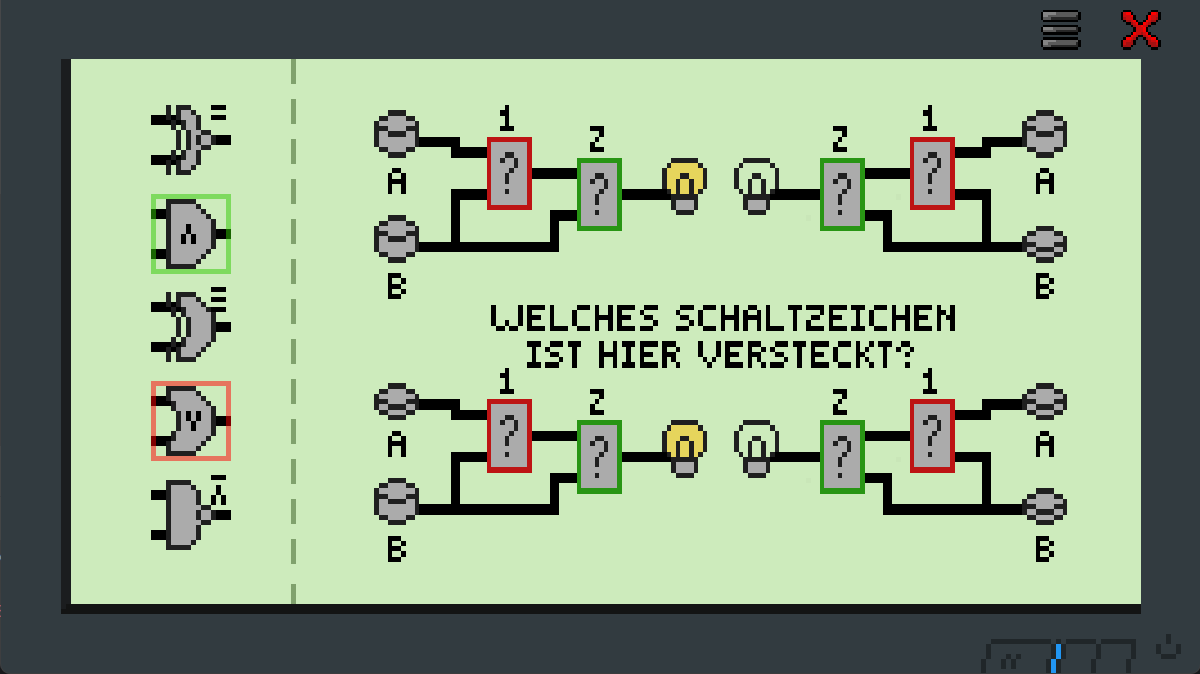
\includegraphics[width=.7\textwidth]{bilder/MinispielInformatik.png}
	\caption{Level 2 des Minispiels der Fachschaft Informatik}
	\label{fig:mginf}
\end{figure}

Verschiedene Schwierigkeiten werden auf zwei Weisen ermöglicht:

\begin{itemize}
    \item Die Anzahl an Logikgattern, aus denen ausgewählt werden kann, erhöht sich mit jedem Schwierigkeitsgrad.
            So sind es im ersten Level 4, im zweiten Level 5 und im dritten Level 6 Logikgatter, welche zur Auswahl stehen.
    \item Die Komplexität des Schaltkreises sowie die Anzahl an verdeckten Gattern ändern sich dem Schwierigkeitsgrad entsprechend.
\end{itemize}

Jedes Level verwendet außerdem, im Sinne der Variabilität, drei verschiedene Schaltkreise, aus denen bei jedem Minispiel-Start einer zufällig gewählt wird.

\subsubsection{Level 1}

Bei den Schaltkreisen des ersten Levels fehlt jeweils nur ein Logikgatter, das zwei Eingänge mit einem Ausgang verbindet.
Gesucht wird also das Logikgatter $G \in \{\land , \lor , \overline{\land}, \overline{\lor}, \veebar, \overline{\veebar}\}$\footnote{$\land = AND,\ \lor = OR,\ \overline{\land} = NAND,\ \overline{\lor} = NOR,\ \veebar = XOR,\ \overline{\veebar} = XNOR$}, welches folgende Bedingungen erfüllt:

\begin{align*}
    x_1 G x_2 = y
\end{align*}

Dadurch, dass jeder Schaltkreis zwei Eingänge und einen Ausgang besitzt, ergeben sich vier mögliche Zustände, die in Form einer Wahrheitswerttabelle dargestellt werden können.
Für die Rätsel des ersten Levels wurden folgende Tabellen festgelegt:

\begin{table}[H]
    \centering
    \begin{minipage}{.33\textwidth}
        $G = \land$\\
        \vfill
        \begin{tabular}{|c|c|c|} 
            \hline
            $x_1$ & $x_2$ & $y$ \\
            \hline\hline
            $0$ & $0$ & $0$ \\
            $0$ & $1$ & $0$ \\
            $1$ & $0$ & $0$ \\
            $1$ & $1$ & $1$ \\
            \hline
        \end{tabular}
    \end{minipage}
    \hfill
    \begin{minipage}{.32\textwidth}
        $G = \lor$\\
        \vfill
        \begin{tabular}{|c|c|c|} 
            \hline
            $x_1$ & $x_2$ & $y$ \\
            \hline\hline
            $0$ & $0$ & $0$ \\
            $0$ & $1$ & $1$ \\
            $1$ & $0$ & $1$ \\
            $1$ & $1$ & $1$ \\
            \hline
        \end{tabular}
    \end{minipage}
    \hfill
    \begin{minipage}{.33\textwidth}
        $G = \overline{\land}$\\
        \vfill
        \begin{tabular}{|c|c|c|} 
            \hline
            $x_1$ & $x_2$ & $y$ \\
            \hline\hline
            $0$ & $0$ & $1$ \\
            $0$ & $1$ & $1$ \\
            $1$ & $0$ & $1$ \\
            $1$ & $1$ & $0$ \\
            \hline
        \end{tabular}
    \end{minipage}
    \caption{Wahrheitswerttabellen für Level 1 des Informatik-Minispiels}
    \label{tab:wwt01}
\end{table}

Diese Tabellen werden den Spielenden, aufgrund der ansprechenderen Gestaltung, in Form einer Abbildung präsentiert, welche die vier Zustände des Schaltkreises darstellt.
Ebenfalls im Sinne der Gestaltung wurde auf die Konvention, die Eingänge auf der linken Seite und die Ausgänge auf der rechten Seite darzustellen, verzichtet.
In der Abbildung \ref{fig:mginf} ist dies beispielhaft anhand eines Rätsels des zweiten Levels zu erkennen.

Dieses Level kann durch das Auswählen eines falschen Gatters verloren werden, das heißt das Minispiel muss neu gestartet werden, um das Lösen durch Raten zu verhindern.
Bei den folgenden Leveln ist dies nicht der Fall, da diese schon komplex genug sind, um Raten zu verhindern.
Ein Verlieren bei Falschauswahl würde das Spielerlebnis nur verschlechtern, da dies hier eher versehentlich geschieht.
\subsubsection{Level 2}

Im zweiten Level bestehen die Schaltkreise ebenfalls aus zwei Eingängen, sowie einem Ausgang.
Der Unterschied zu Level 1 besteht hierbei darin, dass zwei Logikgatter entfernt wurden.
Durch das erste werden beide Eingänge verbunden.
Der dadurch resultierende Ausgang wird im zweiten Logikgatter wieder mit einem der Eingänge verbunden, wodurch der finale Ausgang entsteht.
Außerdem wurde zur Reduzierung der Komplexitität die Einschränkung hinzugefügt, dass sich die Gatter unterscheiden müssen.
Gesucht werden also die Logikgatter $G_1, G_2 \in \{\land , \lor , \overline{\land}, \overline{\lor}, \veebar, \overline{\veebar}\}$, welche folgende Bedingungen erfüllen:

\begin{align*}
    (x_1 G_1 x_2) G_2 x_2 &= y\\
    G_1 &\neq G_2
\end{align*}

Dadurch, dass jeder Schaltkreis auch im zweiten Level zwei Eingänge und einen Ausgang besitzt, ergeben sich wieder vier mögliche Zustände, die in Form einer Wahrheitswerttabelle dargestellt werden können.
Für die Rätsel des zweiten Levels wurden folgende Tabellen festgelegt:

\begin{table}[h!]
    \centering
    \begin{minipage}{.33\textwidth}
        $G_1 = \land$\\
        $G_2 = \overline{\lor}$
        \vfill
        \begin{tabular}{|c|c|c|} 
            \hline
            $x_1$ & $x_2$ & $y$ \\
            \hline\hline
            $0$ & $0$ & $1$ \\
            $0$ & $1$ & $0$ \\
            $1$ & $0$ & $1$ \\
            $1$ & $1$ & $0$ \\
            \hline
        \end{tabular}
    \end{minipage}
    \hfill
    \begin{minipage}{.32\textwidth}
        $G_1 = \lor$\\
        $G_2 = \veebar$
        \vfill
        \begin{tabular}{|c|c|c|} 
            \hline
            $x_1$ & $x_2$ & $y$ \\
            \hline\hline
            $0$ & $0$ & $0$ \\
            $0$ & $1$ & $0$ \\
            $1$ & $0$ & $1$ \\
            $1$ & $1$ & $0$ \\
            \hline
        \end{tabular}
    \end{minipage}
    \hfill
    \begin{minipage}{.33\textwidth}
        $G_1 = \overline{\land}$\\
        $G_2 = \lor$
        \vfill
        \begin{tabular}{|c|c|c|} 
            \hline
            $x_1$ & $x_2$ & $y$ \\
            \hline\hline
            $0$ & $0$ & $1$ \\
            $0$ & $1$ & $1$ \\
            $1$ & $0$ & $1$ \\
            $1$ & $1$ & $1$ \\
            \hline
        \end{tabular}
    \end{minipage}
    \caption{Wahrheitswerttabellen für Level 2 des Informatik-Minispiels}
    \label{tab:wwt02}
\end{table}

Diese Tabellen werden analog zu Level 1 als Abbildungen dargestellt.

\subsubsection{Level 3}

Im dritten Level bestehen die Schaltkreise aus drei Eingängen, einem Ausgang und drei entfernten Logikgattern.
Durch die ersten beiden werden jeweils zwei der Eingänge miteinander verbunden.
Die dadurch resultierenden Ausgänge werden im dritten Logikgatter verbunden, wodurch der finale Ausgang entsteht.
Gesucht werden also die Logikgatter $G_1, G_2, G_3 \in \{\land , \lor , \overline{\land}, \overline{\lor}, \veebar, \overline{\veebar}\}$, welche folgende Bedingungen erfüllen:

\begin{align*}
    (x_1 G_1 x_2) G_3 (x_2 G_2 x_3) &= y\\
    G_1 \neq G_2 &\neq G_3 
\end{align*}

Dadurch, dass jeder Schaltkreis aus drei Eingänge und einen Ausgang besteht, ergeben sich insgesamt acht mögliche Zustände, die in Form einer Wahrheitswerttabelle dargestellt werden können.
Für die Rätsel des dritten Levels wurden folgende Tabellen festgelegt:

\begin{table}[h!]
    \centering
    \begin{minipage}{.33\textwidth}
        $G_1 = \land$\\
        $G_2 = \veebar$\\
        $G_3 = \lor$
        \vfill
        \begin{tabular}{|c|c|c|c|} 
            \hline
            $x_1$ & $x_2$ & $x_3$ & $y$\\
            \hline\hline
            $0$ & $0$ & $0$ & $0$\\
            $0$ & $0$ & $1$ & $1$\\
            $0$ & $1$ & $0$ & $1$\\
            $0$ & $1$ & $1$ & $0$\\
            $1$ & $0$ & $0$ & $0$\\
            $1$ & $0$ & $1$ & $1$\\
            $1$ & $1$ & $0$ & $1$\\
            $1$ & $1$ & $1$ & $1$\\
            \hline
        \end{tabular}
    \end{minipage}
    \hfill
    \begin{minipage}{.32\textwidth}
        $G_1 = \overline{\veebar}$\\
        $G_2 = \land$\\
        $G_3 = \lor$
        \vfill
        \begin{tabular}{|c|c|c|c|} 
            \hline
            $x_1$ & $x_2$ & $x_3$ & $y$\\
            \hline\hline
            $0$ & $0$ & $0$ & $1$\\
            $0$ & $0$ & $1$ & $1$\\
            $0$ & $1$ & $0$ & $0$\\
            $0$ & $1$ & $1$ & $1$\\
            $1$ & $0$ & $0$ & $0$\\
            $1$ & $0$ & $1$ & $0$\\
            $1$ & $1$ & $0$ & $1$\\
            $1$ & $1$ & $1$ & $1$\\
            \hline
        \end{tabular}
    \end{minipage}
    \hfill
    \begin{minipage}{.33\textwidth}
        $G_1 = \veebar$\\
        $G_2 = \lor$\\
        $G_3 = \land$
        \vfill
        \begin{tabular}{|c|c|c|c|} 
            \hline
            $x_1$ & $x_2$ & $x_3$ & $y$\\
            \hline\hline
            $0$ & $0$ & $0$ & $0$\\
            $0$ & $0$ & $1$ & $0$\\
            $0$ & $1$ & $0$ & $1$\\
            $0$ & $1$ & $1$ & $1$\\
            $1$ & $0$ & $0$ & $0$\\
            $1$ & $0$ & $1$ & $1$\\
            $1$ & $1$ & $0$ & $0$\\
            $1$ & $1$ & $1$ & $0$\\
            \hline
        \end{tabular}
    \end{minipage}
    \caption{Wahrheitswerttabellen für Level 3 des Informatik-Minispiels}
    \label{tab:wwt03}
\end{table}

Da die Wahrheitswerttabellen des dritten Levels acht Zustände beinhalten, wird auf die Darstellung jedes einzelnen Zustandes verzichtet und nur der erste Zustand als Schaltkreis abgebildet.
Die anderen werden als Tabelle präsentiert.

\subsubsection{Reflexion}

Bei dem Minispiel der Fachschaft Informatik wird die Theorie spielerisch mit der Praxis verbunden.
Die Spielenden werden mit abstrakten boolschen Operationen sowie mit erwarteten Ergebnissen konfrontiert und können ihre Überlegungen dann anhand von Logikgattern und Schaltkreisen in die Tat umsetzten.
Es fördert vor allem logisches Denken, jedoch auch die Fähigkeit, mit begrenzten Mitteln ein gewünschtes Ergebnis zu erziehlen.
Außerdem regen die Rätsel durch ihre Komplexitität dazu an, Lösungsstrategien zu entwickeln, anstatt Antwortmöglichkeiten einfach auszuprobieren oder gar zu raten.\\
Das erste Level bietet einen guten Einstieg in die Funktionsweise des Spieles, da hier nur die Eigenschaften der einzelnen Gatter abgefragt und diese noch nicht verkettet werden.
Der Schwierigkeitsgrad nimmt im zweiten Level deutlich zu, jedoch kann hier durch Überlegungen, die zur Vereinfachungen des Problemes führen\footnote{Beispielsweise folgende Aussage: \glqq Der Ausgang ist in jedem Fall gleich Eingang 1.\grqq} dennoch gut eine Lösung gefunden werden.
Das dritte Level ist sehr komplex.
Es verlangt das Verbinden dreier Gatter miteinander, was definitiv über den Rahmen eines schnellen Minispiels hinausreicht.
Hier kann zwar analog zu Level 2 vereinfacht werden, jedoch bleibt das Problem dadurch dennoch sehr schwierig.
Eine Mögliche Lösung wäre das Vorgeben eines oder mehrerer Gatter, ähnlich zum in \ref{sec:mathematics} beschriebenen Mathe-Minispiel.
Auch denkbar wäre eine Einschränkung der Antwortmöglichkeiten.
So könnten die richtigen Gatter schon gegeben sein, müssten jedoch noch an die richtige Stelle plaziert werden.\\
Das Minispiel birgt neben der Schwierigkeit auch anderweitig Potential zur Verbesserung.
Die Grafiken der Logikgatter sind schwer zuzuordnen und setzten die Kenntnis ihrer Funktionsweise vorraus.
Dies könnte mit kleinen Erklärtexten oder Beispielabbildungen behoben werden.
Zusätzlich ist das wiederholte Spielen nur begrenzt möglich.
Zwar bieten die verschiedenen Schaltkreise Variabilität, jedoch ist diese aufgrund der Menge an Rätseln sehr eingeschränkt.
Die insgesamt neun Schaltkreise können schnell auswendig gelernt werden, wodurch das Spiel seine Tiefe verliert.
Dies könnte möglicherweise mit zufällig generierten Wahrheitswerttabellen behoben werden.
Jedoch ist dabei zu beachten, dass viele Tabellen keine oder mehrere Lösungen für den gegebenen Aufbau besitzen.
Es würde sich eher anbieten das Grundkonzept zu überarbeiten, da dieses generell wenig Variabilität bietet.

\subsection{Mathematik}
\label{sec:mathematics}

Die grundlegende Idee dieses Minispiels basiert auf dem chinesischen Legespiel \glqq Tangram\grqq\footnote{Seite „Tangram“. In: Wikipedia - Die freie Enzyklopädie. Bearbeitungsstand: 17. Januar 2025, 11:35 UTC. URL: https://de.wikipedia.org/w/index.php?title=Tangram\&oldid=252340816 (Abgerufen: 14. April 2026, 11:30 UTC)}.
Hierbei wird versucht aus gegebenen Steinen eine gegeben Form zu legen.
Die Spielenden haben gewonnen, wenn die Form zu 95\% mit Steinen bedeckt ist, um das Spielerlebnis angenehmer zu gestalten, da die Steine so nicht exakt am richtigen Platz liegen müssen.
Diese Überprüfung soll automatisch beim Platzieren der Steine ablaufen, um so das Drücken eines \glqqÜberprüfungs\grqq{}-Knopfes zu ersparen.
Das Minispiel kann nicht verloren werden.\\
Die Level der Fachschaft Mathematik bestehen ebenfalls aus zwei wesentlichen Komponenten:
Zunächst gibt es einen Satz an Tangram-Steinen, welche durch Verschieben und Rotieren in eine vorgegebene Silhouette, welche die zweite Komponente darstellt, gelegt werden müssen.
Außerdem werden zufällig gewählte Steine bereits an die richtige Position platziert, um das Lösen zu vereinfachen.

\begin{figure}[H]
	\centering
	\includegraphics[width=.7\textwidth]{bilder/MinispielMathematik.png}
	\caption{Level 2 des Minispiels der Fachschaft Mathematik}
	\label{fig:mgma}
\end{figure}


Verschiedene Schwierigkeiten werden auf zwei Weisen ermöglicht:

\begin{itemize}
    \item Die Anzahl an bereits richtig angeordneten Tangram-Steinen, verringert sich mit jedem Schwierigkeitsgrad.
            So sind es im ersten Level zwei vorgegebene Steine, im zweiten Level ein und im dritten Level kein vorgegebener Stein.
    \item Die Komplexitität der Silhouette ändert sich dem Schwierigkeitsgrad entsprechend.
\end{itemize}

Jedes Level verwendet außerdem, im Sinne der Variabilität, drei verschiedene Silhouetten, aus denen bei jedem Minispiel-Start eine zufällig gewählt wird.

\subsubsection{Level 1}

Im folgenden sind die Puzzle des ersten Levels mit einer beispielhaften Lösung abgebildet.

\begin{figure}[H]
    \centering
    \begin{minipage}{0.33\textwidth}
        
\includegraphics[width=1\textwidth]{bilder/TangramHerz.png}
        \caption{Herz}
        \label{fig:therz}
    \end{minipage}
    \hfill
    \begin{minipage}{0.32\textwidth}
        
\includegraphics[width=1\textwidth]{bilder/TangramSchwan.png}
        \caption{Schwan}
        \label{fig:tschwan}
    \end{minipage}
    \hfill
    \begin{minipage}{0.33\textwidth}
        
\includegraphics[width=1\textwidth]{bilder/TangramBerg.png}
        \caption{Berg}
        \label{fig:tberg}
    \end{minipage}
\end{figure}

\subsubsection{Level 2}

Im folgenden sind die Puzzle des zweiten Levels mit einer beispielhaften Lösung abgebildet.

\begin{figure}[H]
    \centering
    \begin{minipage}{0.33\textwidth}
        
\includegraphics[width=1\textwidth]{bilder/TangramHaus.png}
        \caption{Haus}
        \label{fig:thaus}
    \end{minipage}
    \hfill
    \begin{minipage}{0.32\textwidth}
        
\includegraphics[width=1\textwidth]{bilder/TangramNinjastern.png}
        \caption{Ninjastern}
        \label{fig:tninjastern}
    \end{minipage}
    \hfill
    \begin{minipage}{0.33\textwidth}
        
\includegraphics[width=1\textwidth]{bilder/TangramBaum.png}
        \caption{Baum}
        \label{fig:tbaum}
    \end{minipage}
\end{figure}

\subsubsection{Level 3}

Im folgenden sind die Puzzle des dritten Levels mit einer beispielhaften Lösung abgebildet.

\begin{figure}[H]
    \centering
    \begin{minipage}{0.33\textwidth}
        
\includegraphics[width=1\textwidth]{bilder/TangramLäufer.png}
        \caption{Läufer}
        \label{fig:tlaeufer}
    \end{minipage}
    \hfill
    \begin{minipage}{0.32\textwidth}
        
\includegraphics[width=1\textwidth]{bilder/TangramKamel.png}
        \caption{Kamel}
        \label{fig:tkamel}
    \end{minipage}
    \hfill
    \begin{minipage}{0.33\textwidth}
        
\includegraphics[width=1\textwidth]{bilder/TangramHai.png}
        \caption{Hai}
        \label{fig:thai}
    \end{minipage}
\end{figure}

\subsubsection{Reflexion}

Das Minispiel der Fachschaft Mathematik nutz das seit Jahrhunderten bewährte chinesische Legespiel \glqq Tangram\grqq{} um das räumliche Denken der Spielenden auf die Probe zu stellen.
Es mag sehr simple erscheinen, besitzt jedoch viele mathematische Rafinessen, welche teilweise auch in unserem Schulhaus beleuchtet werden. 
Es fördert neben dem bereits Genannten ebenfalls die Fähigkeit Strukturen zu erkennen und diese zu verallgemeinern.
Die meißten Tangramsteine können als eine Kombination anderer dargestellt werden, wodurch sowohl Vielfalt, als auch Restriktion entsteht.
Sollte beispielsweise ein großer Stein übrig sein, jedoch nur kleine freie Plätze, kann versucht werden bereits platzierte Steine durch den Übrigen zu ersetzten und mit den frei gewordenen Steinen die Lücken zu füllen.\\
Die einzelnen Level unterscheiden sich wenig voneinander.
Die Schwierigkeit des Lösens eines einzelnen Puzzles ist sehr subjektiv und lässt sich so schwer festlegen, weswegen die Zuteilung der Puzzle zu den jeweilligen Level nicht sinnvoll ist.
Besser wäre es diese Levelübergreifend zu definieren und so die Schwierigkeit nur durch die Anzahl der vorgegebenen Steine zu differenzieren.
Jedoch wirft auch dies Probleme auf:
Die Schwierigkeitsänderung zwischen den Leveln ist eher gering.
So kann es beispielsweise vorkommen, dass der im zweiten Level bereits platzierte Stein so gegeben ist, dass die Platzierung eines zweiten offensichtlich erscheint\footnote{Beispielsweise das Quadrat in Abbildung \ref{fig:tninjastern}, welches die Platzierung des orangenen Dreiecks vorgeben würde.}, wodurch das Lösen des Puzzles nicht schwerer, als im ersten Level ist.
Außerdem ist diese Art des Erschwerens nicht beliebig skalierbar, da nicht weniger als kein Stein vorgegeben werden kann.\\
Das dritte Level entspricht nicht vollständig dem Bild einer schwierigen Herausforderung, weil es sich, wie bereits genannt, wenig von den anderen Leveln unterscheidet und das Lösen auch etwas zu einfach ist.
Es müsste also erschwert werden, was durch das aktuelle System nicht gewährleistet werden kann.
Eine mögliche Lösung wäre das Einführen eines zweiten Tangram-Sets, wodurch deutlich komplexere Figuren möglich werden und so auch der Unterschied zu den vorherigen Schwierigkeitsgraden deutlich wird. 

\section{Item- und Charakterdesign}
Zu Beginn der Projektarbeit haben wir, Wuyi und Arthur, uns zusammengesetzt und die Aufgaben, die uns als Gruppe \emph{Item- und Charakterdesign} zugeteilt wurden, klar definiert. Die Aufgaben sind folgende:

\begin{itemize}
	\item Festlegen der Anzahl an Lehrern und Items, sowie Auswählen der im Spiel vertretenen Lehrer für die jeweiligen Fachschaften
	\item Zeichnen der Spielerfigur sowie der Lehrer und im Spiel benutzten Items
	\item Implementieren des Spielers, der Lehrer und Items in das Programm 
\end{itemize}

\subsection{Spielerfigur}
Die Spielerfigur soll einerseits visuell den Benutzer im Spiel involvieren. Dafür gibt es über ein Menü die Möglichkeit, Haare, Hautfarbe und Kleidung individuell einzufärben.

Anderseits stellt sie den Hauptcharakter des Spieles dar und besitzt dementsprechend Funktionen, welche den Kampf gegen die Lehrer ermöglichen, wie auch ein Inventar, in welchem die erhaltenen Items gespeichert und mit Bild und Namen angezeigt werden. Dieses kann durch Anklicken der Spielerfigur geöffnet und mit einem Button wieder geschlossen werden. Die für den Kampf relevanten Funktionen wurden mit Absprache von der Gruppe \emph{Kampfkonzept} eingefügt und lagen außerhalb unserer Zuständigkeit.

\subsection{Lehrer*innen}
Die Lehrer und Lehrerinnen treten im Spiel als Antagonisten auf, die es zu besiegen gilt. Geplant waren 3 Lehrer*innen pro Fachschaft mit variierenden Schwierigkeitsgraden im Kampf. Um diese darzustellen, braucht es sowohl ein Bild des Lehrers/der Lehrerin, als auch Eigenschaften wie einen Namen, den Schwierigkeitsgrad oder das \glqq{}Level\grqq{}, die Zugehörigkeit zu einer Fachschaft, eine Menge an Lebenspunkten sowie eine Auswahl von Items, welche im Kampf zur Verfügung stehen.

\subsection{Items}
Die Items sind gebräuchliche Gegenstände/Materialien des Schulalltages oder auch bekannte Modelle/Konzepte der MINT-Fächer und erfüllen die Rolle von Waffen und Belohnungen im Spiel, die durch das erfolgreiche Beenden von Minispielen oder Besiegen von Lehrern nach einem Duell gewonnen und im Kampf gegen selbige auch eingesetzt werden können. Jedes Item besitzt einen Namen, ein Bild, welches im Spiel angezeigt wird, und einen Stärkegrad oder \glqq{}Level\grqq{}, das den Schaden im Kampf bestimmt. Es gibt 30 Items, sechs pro Fachschaft, mit jeweils zwei Items der Stärke null, zwei der Stärke eins und zwei der Stärke zwei. Nach dem Abschluss eines Minispiels erhält der Spieler ein Item der Fachschaft, zu dem das Spiel gehört. Der Stärkegrad des erhaltenen Items entspricht dabei dem Schwierigkeitsgrad jenes Spiels. Das heißt, je schwerer das Minispiel, desto höher ist das Level des erhaltenem Items.


\section{Sound}
Java bietet über die \texttt{Java Sound API} eine vorgefertigte Schnittstelle zum Laden und Abspielen von Audiodateien.
\par Die am einfachsten zu verwendende Klasse dieser Schnittstelle ist
\texttt{javax.sound.sampled.Clip}. Diese bietet Methoden wie \texttt{setMicrosecondPosition}, \texttt{start} und \texttt{stop}, mit
welchen die Wiedergabe einfach gesteuert werden kann. Der entscheidende
Nachteil der \texttt{Clip}-Klasse ist jedoch, dass sie die gesamten Audiodaten auf einmal in den Speicher lädt. Das ist bei kleinen, wenige Sekunden langen Audiodateien kein Problem, jedoch für Musikstücke, welche mehrere Minuten dauern, ungeeignet. 
\par Um dieses Speicherproblem zu lösen, müssen die Audiodaten \textit{gestreamt},
also in kleinen Stücken in den Speicher geladen, abgespielt und wieder
verworfen werden. Es befindet sich also immer nur eine kleine Teilmenge der Gesamtaudiodaten im Speicher.
\par Zur Umsetzung des Streamens stellt die Java-Standardbibliothek die Klassen \texttt{AudioInputStream} und \texttt{SourceDataLine} bereit. Erstere ermöglicht es, eine Audiodatei zu öffnen und zu
dekodieren, also die enthaltenen Audiodaten zu lesen. Im zweiten
Schritt müssen die gelesenen Daten an eine Instanz von \texttt{SourceDataLine} übergeben werden, welche diese dann abspielt. Dazu wird deren \textit{write}-Methode verwendet.

Zusätzlich sollte es möglich sein, Sounds in Gruppen zusammenzufassen,
um sie gemeinsam starten, pausieren und stoppen zu können.

\chapter{Programmdokumentation}

Im Abschnitt \emph{Programmdokumentation} soll der Aufbau und die Struktur des Programms dargelegt werden, also wie die Lösungsidee im Programm umgesetzt wurde. Die Erläuterung der wichtigsten Funktionen und Klassen des Programms soll zusätzlich durch relevante Ausschnitte von kommentierten Quelltexten, Struktogramme und/oder Pseudocode-Beschreibungen von wesentlichen Teilalgorithmen veranschaulicht werden.


Das CZGame ist ein am Carl-Zeiss-Gymnasium Jena orientiertes, als Point- \& Click ausgelegtes Spiel. Ziel ist es sich gegen alle Lehrer aus den verschiedenen Fachschaften durchzusetzen. Dabei wird man im Verlauf des Spiels immer besser und bekommt immer stärkere Attribute. \\

\begin{figure}[h!]
    \centering
    \includegraphics[width=0.5\linewidth]{bilder/StartSzene.png}
    \caption{Die Startszene des CZGame}
    \label{fig:placeholder}
\end{figure}

Das Spiel startet in einer Szene, die dem Foyer der Schule ähnelt. Von hier aus kann man sich mithilfe der Pfeile fortbewegen. Man kann entweder nach links und rechts um in die verschiedenen Gänge der Fachschaften zu gelangen, oder man geht die Treppe in die nächste Etage hinauf. In den Gängen der Fachschaften kann man nun Minigames finden. Diese beinhalten 3 unterschiedlich schwere Level (leicht, mittel, schwer). Die Minigames sind an die jeweilige Fachschaft angelegt. Beispielsweise muss man in der Informatik Logische Schaltungen durchblicken, während der Spieler in der Chemie mit dem sortieren von verschiedenen Flüssigkeiten konfrontiert wird. Schafft man es die Minigames erfolgreich zu lösen, erhält man verschiedenste Items, die einem im Kampf gegen die Lehrer unterstützen. \\
In den Gängen kann man außerdem in die Räume gehen. Dafür genügt es, wenn man die Tür anklickt. In den Räumen findet man die verschieden Lehrer. Möchte man sich im Kampf gegen diese Beweisen muss man einmal auf den Lehrer klicken. \\
Der Kampf basiert auf verschiedenen Runden. Lehrer und Schüler versuchen abwechseln sich ihrem gegenüber zu beweisen. Durch die Items kann man stärker werden und die Lehrer leichter besiegen. Dabei muss der Spieler jedoch aufpassen, denn nicht jedes Item hilft bei jedem Lehrer gleich viel. 



\section*{Quelltexte}
Für Quelltexte eignet sich das Paket \texttt{listings}.

\begin{lstlisting}[caption=Beispiel, label=lst:beispiel, captionpos=b, language=Java]
public class Test {
	/**
	* Hilfreiche Kommentare machen Lesende gluecklich.
	*/
	public static void main(String[] args) {
		int xVar = 0;
		for (int i = 0; i <= 11; i+=1) {
			xVar = 3 + xVar;
		}
		System.out.println(i +" * 3 = " + xVar);
	}
}
\end{lstlisting}

\section*{Struktogramme}
Struktogramme können in \texttt{Structorizer} umgesetzt und dann als pdf-Datei exportiert werden. Das Programm \texttt{Structorizer} exportiert das Struktogramm als vollständige Seite (siehe links in der Abbildung \ref{fig:pdfs}. 
Es muss noch beschnitten werden. Als Online-Tool eignet sich \url{https://pdfresizer.com/crop}.
\begin{enumerate}
	\item Datei auswählen (Choose files)
	\item Hochladen (Upload)
	\item Am Ende der "`neuen"' Webseite ganz unten bei Action: \texttt{Autocrop} auswählen und dann den Button \texttt{Crop It} wäheln und ins speichern. Die beschnittene Datei befindet sich nun im Downloadordner.
\end{enumerate}
\begin{figure}[h!]
	\centering
	\begin{minipage}{.45\textwidth}
		\fbox{\includegraphics[scale=.3]{bilder/test.pdf}}
	\end{minipage}
	\hfill
	\begin{minipage}{.45\textwidth}
		\fbox{\includegraphics[scale=.3]{bilder/test-crop.pdf}}
	\end{minipage}
	\caption{unbeschnittenes und beschnittenes PDF}
	\label{fig:pdfs}
\end{figure}

\section*{Formale Beschreibungen von Teilalgorithmen}
Pseudocode eines Algorithmus sollte in einer \texttt{verbatim}-Umgebung erfolgen:
\begin{verbatim}
 Initialisiere xVar mit 0
 FÜR i=1 BIS 11
    xVar = 3 * xVar
 Ausgabe: xVar
\end{verbatim}

\section{Engine}
\begin{sloppypar}

\subsection{Fenster}

Die Klasse \texttt{czg.MainWindow} stellt das Spielfenster
dar und beinhaltet die \texttt{main}-Methode sowie eine
Reihe von statischen Konstanten. Letztere werden in der
Dokumentation mit dem gleichen Namen wie im Code bezeichnet.

\begin{itemize}
	\item \texttt{int PIXEL\_SCALE}: Da das Spiel im Pixel-Art-Stil
	      umgesetzt wurde, sind die im Spiel enthaltenen Bilddateien sehr
	      klein. Deshalb werden sie um diesen konstanten Faktor skaliert.
	\item \texttt{int WIDTH, HEIGHT}: Die Höhe und Breite des Spielfensters
	      in Pixeln.
	\item \texttt{int FPS}: Abkürzung für \textit{Frames per Second}.
	      Wie oft Spiellogik und Rendern in einer Sekunde ausgeführt
	      werden sollen.
	\item \texttt{MainWindow INSTANCE = new MainWindow()}: Die \textit{Singleton}-
	      Instanz des Fensters.
	\item \texttt{long TIME\_AT\_UPDATE\_START}: Der Wert von \texttt{System.nanoTime()}
	      zu beginn eines Logik-Durchlaufs. Siehe Abschnitt \ref{programm:engine:eingabe}.
\end{itemize}


\subsubsection{\texttt{main}-Methode}

\texttt{czg.MainWindow.main} erledigt folgende Initialisierungsaufgaben:

\begin{itemize}
	\item Platzieren das Fenster in der Mitte des Bildschirms und
	      Anzeigen desselben
	\item Starten der Hintergrundmusik, indem eine neue Instanz von
	      \texttt{czg.sound.StreamSound} zur globalen Sound-Gruppe
	      \texttt{czg.sound.SoundGroup.GLOBAL\_SOUNDS} hinzugefügt wird.
	      Siehe Abschnitt \ref{programm:engine:sound:gruppe}.
	\item Korrigieren der Fenstergröße. Dies ist notwendig, da beim
	      Aufruf von \texttt{javax.swing.JFrame.setSize} die vom
	      Betriebssystem angezeigte Fensterleiste mit einberechnet
	      ist. Entsprechend muss die Höhe des Fensters noch einmal
	      um die Höhe der Fensterleiste erhöht werden, um keinen Teil
	      der Grafik abzuschneiden.
	\item Anzeigen der ersten Szene, indem eine neue Instanz der entsprechenden
	      Klasse zum Szenenstapel hinzugefügt wird. Siehe Abschnitt \ref{programm:engine:szene:stapel}.
	\item Starten der Hauptschleife. Siehe Abschnitt \ref{programm:engine:hauptschleife}.
\end{itemize}


\subsubsection{Hauptschleife} \label{programm:engine:hauptschleife}

Wie in Abschnitt \ref{idee:engine:hauptschleife} erwähnt läuft die
Hauptschleife mit einer Frequenz von 60Hz, wie in \texttt{czg.MainWindow.FPS}
definiert. Die Grundidee des Algorithmus findet sich ebenfalls dort.
Im folgenden ist die letztendliche Implementierung in \texttt{MainWindow.java}
gelistet:

\begin{lstlisting}[caption=Hauptschleife, label=programm:engine:hauptschleife:code, captionpos=t, language=Java]
// In welchem Zeitintervall (in Nanosekunden) die Spiellogik
// ausgeführt werden soll
final double interval = 1e9 / FPS;
// Zählt, wie oft die Spiellogik durchlaufen werden sollte.
double delta = 0;

// Zeit seit dem letzten Durchlauf der while(true)-Schleife
long lastTime = System.nanoTime();
// Zweite Zeit-Variable. Wird zur neuen lastTime.
long currentTime;

//noinspection InfiniteLoopStatement
while(true) {
	// Aktuelle Zeit messen
	currentTime = System.nanoTime();
	
	// Die Zeit berechnen, die seit dem letzten Durchlauf
	// dieser Schleife vergangen ist.
	// Damit berechnen, wie oft die Spiellogik in dieser
	// Zeitspanne hätte durchlaufen
	// werden sollen (normalerweise eine Anzahl <1).
	delta += (currentTime - lastTime) / interval;
	
	// Die currentTime wird wieder zur lastTime
	lastTime = currentTime;
	
	// Alle nötigen Durchläufe abarbeiten
	while(delta >= 1) {
		TIME_AT_UPDATE_START = System.nanoTime();
		
		// Code für Szenen und Objekte ausführen
		SceneStack.INSTANCE.update();
		
		[ausgelassen]
		
		// Grafik
		SceneStack.INSTANCE.repaint();
		
		// Zusätzliche Aktualisierung
		// für die Eingabeverarbeitung
		Input.INSTANCE.update();
		
		// Durchlauf abgeschlossen, Zähler kann um
		// 1 verringert werden
		delta--;
	}
}
\end{lstlisting}

Der hier ausgelassene Teil des Codes beinhaltet lediglich
die Logik für einige Tastenkürzel. Diese werden in
späteren Abschnitten an den entsprechenden Stellen
erwähnt und sind im Programmablaufprotokoll noch einmal
gelistet.


\subsection{Eingabe} \label{programm:engine:eingabe}

Die Klasse \texttt{czg.util.Input} implementiert die in
\ref{idee:engine:grafik-eingabe} erwähnten Interfaces
\texttt{java.awt.event.KeyListener} und \texttt{java.awt.event.MouseListener},
sowie zusätzlich noch \texttt{java.awt.event.FocusListener}.
Zusätzlich definiert sie die Konstante \texttt{HELD\_THRESHOLD}.
Diese sagt aus, wie lange eine Taste gedrückt sein darf und
dabei noch als gedrückt und nicht als gehalten gilt.
Die Verwendung dieser Konstante sowie die verschiedenen
Zustände von Tasten werden im Verlauf dieses Abschnitts
näher erklärt.

Der Konstruktor der Klasse ist privat. Es kann jedoch
über die statische Konstante \texttt{Input.INSTANCE}
auf eine Singleton-Instanz der Klasse zugegriffen werden.
Diese wird u.A. von \texttt{MainWindow} an deren
\texttt{addKeyListener}- und \texttt{addMouseListener}-Methoden
übergeben, um das Eingabeverarbeitungssystem funktionstüchtig
zu machen.


\subsubsection{Speichern von gedrückten Tasten}

Den Kern der \texttt{Input}-Klasse bilden zwei Instanzen von
\texttt{java.util.concurrent.ConcurrentHashMap}:
\texttt{keyStates} und \texttt{mouseStates}.
Wird eine Taste gedrückt, werden die entsprechenden
Methoden \texttt{keyPressed} und \texttt{mousePressed} von
\texttt{Swing} aufgerufen. Die Implementierungen dieser
Methoden in \texttt{Input} ordnen dann dem Tasten-Code der
gedrückten Taste, welcher über die \texttt{getKeyCode}-Methode
des \texttt{KeyEvent}- bzw. \texttt{MouseEvent}-Objekts,
welches an die Methode übergeben wird, erhalten werden kann,
den aktuellen Wert von \texttt{System.nanoTime()} zu, speichern
also den Zeitpunkt, an welchem die Taste gedrückt wurde.

Analog wird ein Eintrag in der entsprechenden \texttt{ConcurrentHashMap}
wieder entfernt, wenn die zugehörige Taste losgelassen und
somit \texttt{Input.keyReleased} bzw. \texttt{Input.mouseReleased}
aufgerufen wird.

Befindet sich das Spielfenster nicht mehr im Vordergrund bzw. im Fokus,
so ruft \texttt{Swing} die Methode \texttt{focusLost} aus dem \texttt{FocusListener}-Interface
auf. Die Implementierung dieser Methode in \texttt{Input} besteht
daraus, alle Einträge aus den beiden \texttt{ConcurrentHashMap}s zu
entfernen.


\subsubsection{Tastenzustände und das Abfragen dieser}

Nun kann der Zustand einer Taste mittels den Methoden
\texttt{Input.getKeyState(int)} und \texttt{Input.getMouseState(int)}
abgefragt werden. Die zu übergebenden Parameter sind die
Tasten-Codes der abzufragenden Maus- oder Tastaturtaste,
welche als statische Konstanten in den bereits erwähnten
Klassen \texttt{KeyEvent} und \texttt{MouseEvent} definiert sind.

Die beiden Methoden geben eine Konstante aus dem Enum
\texttt{Input.KeyState} zurück. Dieses definiert genau
drei Zustände für Tasten:

\begin{itemize}
	\item \texttt{NOT\_PRESSED}: Die Taste ist nicht gedrückt
	\item \texttt{PRESSED}: Die Taste wurde, von \texttt{MainWindow.TIME\_AT\_UPDATE\_START}
	      aus gemessen, höchstens für die Länge des Zeitintervalls
	      \texttt{Input.HELD\_THRESHOLD} gedrückt.
	\item \texttt{HELD}: Ist eine Taste schon länger gedrückt
	      als \texttt{Input.HELD\_THRESHOLD}, gilt sie als gehalten
	      und nicht mehr als gedrückt.
\end{itemize}

Zusätzlich bietet \texttt{KeyState} die Methode \texttt{isDown},
welche \texttt{true}, wenn es sich bei der Enum-Konstante,
für welche die Funktion aufgerufen wurde, um \texttt{PRESSED}
oder \texttt{HELD} handelt, und sonst \texttt{false} zurückgibt.

Die von \texttt{Input.getKeyState(int)} verwendete
statische Methode \texttt{KeyState.fromTimePressed(long)} verlangt
als Parameter den Zeitpunkt, an dem die Taste gedrückt wurde, also
\texttt{keyPressed} bzw. \texttt{mousePressed} aufgerufen wurde,
leitet daraus die passende Enum-Konstante ab und gibt sie zurück.

Wie im Programmcodelisting \ref{programm:engine:hauptschleife:code} der Hauptschleife
zu sehen ist, wird als letzter Teil jedes Frames die Methode
\textit{Input.update} aufgerufen. Dies hängt zusammen mit den
internen Listen \texttt{Input.keyButtonsToUpdateToHeld} und
\texttt{Input.mouseButtonsToUpdateToHeld}: Jedes mal, wenn
\texttt{Input.getKeyState} bzw. \texttt{Input.getMouseState}
feststellt, dass der Zustand einer Taste \texttt{PRESSED} ist,
wird deren Tasten-Code zu der entsprechenden Liste hinzugefügt.
Beim Aufruf von \texttt{Input.update} werden dann alle Einträge
für die Tasten-Codes in den Listen in der entsprechenden Map
zu \texttt{HELD} geändert - wurde eine Taste also in einem Frame
abgefragt und galt als \texttt{PRESSED}, so gilt sie ab dem nächsten
Frame immer als \texttt{HELD}, egal wie lange sie eigentlich gehalten
wurde. So werden z.B. Mausklicks nicht über mehrere Frames hinweg
mehrfach registriert, denn die entsprechende Maustaste kann nur
für höchstens einen Frame als \texttt{PRESSED} gelten.


\subsubsection{Mausposition}

Außerdem speichert \texttt{Input} die Position des Mauszeigers
sowie diese im vorangegangenen Frame. Dies ist gelöst mithilfe
zweier privater Variablen \texttt{mousePosition} und
\texttt{lastMousePosition}, deren Werte über entsprechende
Getter-Methoden abgefragt werden können. Beim Aufruf von
\texttt{Input.update} erhält \texttt{lastMousePosition} den
Wert von \texttt{mousePosition}. Letztere bekommt dann einen
neuen Wert, welcher mit der \texttt{getMousePosition}-Methode
des Szenenstapels erhalten wird, da dieser \texttt{javax.swing.JPanel}
erweitert. Siehe \ref{programm:engine:szene:stapel}. Würde
stattdessen die Methode mit dem gleichen Namen von \texttt{MainWindow}
aufgerufen werden, so wäre die Mausposition versetzt, da der
Ursprung der von dieser Methode zurückgegebenen Koordinaten
bei der oberen linken Ecke des Fensters \textbf{inklusive Titelleiste}
liegt.



\subsubsection{Debugging-Modus}

Durch wiederholtes Drücken der Taste \texttt{D} kann 


\subsection{Spiel-Objekte}

Spiel-Objekte werden mithilfe der Klasse \texttt{czg.objects.BaseObject}
umgesetzt. Diese speichert folgende Eigenschaften:

\begin{itemize}
	\item X- und Y-Koordinaten, in Pixeln. Dabei ist $(0|0)$ die
		  obere linke Ecke des Spielfensters, und die Koordinaten
		  steigen nach unten bzw. nach rechts in positive Richtung an.
	\item Höhe sowie Breite des Objekts, in Pixeln
	\item Ein Bild, welches an den Koordinaten und mit der Größe
	      des Objekts gezeichnet werden soll. Dieses kann auch
	      \texttt{null} sein, in diesem Fall ist das Objekt
	      unsichtbar.
\end{itemize}

Diese sind alle als \texttt{public} deklariert, können also
von jeder Stelle im Code aus gelesen und geändert werden.

Die Klasse bietet drei Konstruktoren, welche verschiedene
Teilmengen der oben gelisteten Eigenschaften als Parameter
annehmen: Entweder nur ein Bild, ein Bild und eine Position,
oder alle drei Eigenschaften. Werden Höhe und Breite nicht
explizit angegeben, werden sie auf die Höhe und Breite des
Bildes, jeweils mit \texttt{PIXEL\_SCALE} multipliziert,
gesetzt. Wird keine Position angegeben, wird das Objekt
in die Mitte des Spielfensters platziert.

Weiterhin definiert \texttt{BaseObject} eine Reihe an
Methoden:

\begin{itemize}
	\item \texttt{getHitbox}: Verpackt Position und Größe in ein
	      \texttt{java.awt.geom.Rectangle2D}-Objekt, welches eine
	      Reihe nützlicher Methoden bietet.
	\item \texttt{isClicked(boolean includeTransparency)}: Prüft,
	      ob das Objekt angeklickt wurde, also ob sich der Mauszeiger
	      über dem Objekt befindet und die linke Maustaste gedrückt
	      ist. Der optionale Parameter \texttt{includeTransparency}
	      gibt an, ob auch ein Klick auf transparente Bereiche
	      des Bildes des Objektes berücksichtigt werden soll.
	\item \texttt{draw(Graphics2D)}: 
\end{itemize}


\subsection{Szenen}

\subsubsection{Der Szenenstapel} \label{programm:engine:szene:stapel}


\subsection{Sound}

Die \texttt{Java Sound API} untersetützt standardmäßig nur das unkomprimierte \texttt{WAV}-Format. Die Audiodateien liegen allerdings 
aus Gründen der effizienteren Speicherplatznutzung im komprimierten \texttt{Ogg/Vorbis}-Format vor. Um diese laden zu können

\subsubsection{Sound-Gruppe} \label{programm:engine:sound:gruppe}

\end{sloppypar}

\section{Grafikdesign}
\input{texte/04_programmdoku-Grafikdesign.tex}

\section{Kampfkonzept}
Zur Implementierung wurden jeweils im SchülerObject und im LehrerObject zwei Funktionen (nämlich angriff() und verteidigung()) und eine KampfScene angelegt.\\
Außerdem wurde ein Hintergrund für die KampfScene gepixelt.\\

\subsubsection{KampfScene}

Die KampfScene ist der Grundbaustein für die Kämpfe. Sie ist einerseits das Szenenbild, in dem sich der Schüler und der Lehrer befinden, andererseits ist sie aber auch zur Verwaltung des Kampfes da.\\
Am Anfang wird in dieser das Hintergrundbild initialisiert, dann der Lehrer und der Schüler. (Beim Lehrer werden dafür die Leben auf den richtigen Wert gesetzt, die Items werden ihm gegeben und seine Instanz wird erstellt. Beim Schüler muss deutlich weniger getan werden, weil seine Instanz schon existiert. Es werden nur seine Leben festgesetzt.) Diese beiden werden auch an ihrer richtige Position im Bild gesetzt.\\
Danach fängt eine while Schleife an, die so lange läuft, bis eine der beiden Parteien null Lebenspunkte haben. Außerdem kann der Spieler sich jederzeit mit einem Klick auf den Button \glqq Aufgeben \grqq dazu entscheiden den Kampf zu beenden.\\
In dieser wechseln sich die Angriffsfunktionen des Schülers und des Lehrers immer wieder ab.

\subsubsection{Angriff()}

Der Schüler kann zuerst auf sein Inventar zugreifen und sich eins seiner Items aussuchen. Das Level dieses Items wird dann im integer level gespeichert und es wird lehrer.verteidigung(level) aufgerufen, damit der Lehrer auf das ausgesuchte Item reagieren kann.\par
Wenn der Lehrer angreift, wird mit random.nextInt() ein Item ausgesucht, das Level im integer level gespeichert und danach PlayerObject.INSTANCE.verteidigung(level) aufgerufen. Dabei sind die Wahrscheinlichkeiten für jedes der 4 Items des Lehrers gleich, also je 25\%.
\begin{lstlisting}
	// Der Lehrer wählt random, welches der Items er zum Angreifen benutzt. 
	Random rand = new Random();
	int move = rand.nextInt(4);
	int level;
	ItemType item_lehrer;
	
	item_lehrer = lehrer_items.get(move);
	level = item_lehrer.LEVEL;
	
	PlayerObject.INSTANCE.verteidigung(level);
\end{lstlisting}

\subsubsection{Verteidigung()}

Wenn der Schüler verteidigen muss, kann er sich eins seiner Items aus dem Inventar aussuchen. Danach wird der Schaden wie in der Lösungsidee berechnet. Danach werden die Lebenpunkte des Schülers gegebenfalls um den Schaden vermindert.\par
Wenn der Lehrer verteidigen muss, wählt er mit random.nextInt() aus, welches Item er verwenden will oder, ob er nichts tun wird. Auch sind die Wahrscheinlichkeiten für alle Items gleich, aber es gibt noch die fünfte Option des Nichtstuns, deshalb ist die Wahrscheinlichkeit für jede der fünf Optionen 20\%. Danach wird wieder der Schaden berechnet und dann von den Lebenspunkten des Lehrers abgezogen. 
\begin{lstlisting}
	// Es wird random ausgewählt, ob ein Item gewählt wird (und welches), oder ob der Lehrer nichts macht.
	Random rand = new Random();
	int move = rand.nextInt(5);
	int schaden;
	ItemType item_lehrer;
	
	// Falls die Null genommen wurde, wird kein Item vom Lehrer benutzt.
	if (move == 0) {
		schaden = level;
	}
	else {
		item_lehrer = lehrer_items.get(move - 1);
		schaden = level - item_lehrer.LEVEL;
		if (schaden <= 0) {
			schaden = 0;
		}
		
	}
	
	hp -= schaden;
\end{lstlisting}


\section{Minigames}
Da die Minispiele alle einem ähnlichen Grundaufbau folgen, bietet es sich an, diesen objektorientiert und modular zu implementieren, um Redundanz zu vermeiden.
Dieser Grundaufbau besteht aus den folgenden Klassen:

\begin{itemize}
    \item \texttt{LevelScene}
    \item \texttt{LevelSelectorScene}
    \item \texttt{MinigameEndScene}
    \item \texttt{Minigames}
\end{itemize}

\paragraph{LevelScene} Diese abstrakte Klasse ist eine Erweiterung der \texttt{BaseScene} und stellt allgemeine Variablen und Methoden zur Verfügung.
Sie beinhaltet:

\begin{sloppypar}
    \begin{itemize}
        \item \texttt{REWARD}: Ein \texttt{ItemObject}, welches die Spielenden nach erfolgreichendem Beenden des Levels erhalten.
            Es wird mit Hilfe der Methode \texttt{getMinigameReward} der \texttt{ItemObject}-Klasse generiert.
        \item Ein \texttt{BackdropObject} welches das zur Fachschaft gehörende Hintergrundbild beinhaltet.
        \item \texttt{exitButton}: Ein \texttt{ButtonObject}, welches das Verlassen des Minispiels mittels Entfernen der obersten zwei Scenen des \texttt{SceneStack}, hier \texttt{LevelScene} und \texttt{LevelSelectorScene}, ermöglicht.
        \item \texttt{menuButton}: Ein \texttt{ButtonObject}, welches die Rückkehr zur Level-Auswahl mittels Entfernen der obersten Scene des \texttt{SceneStack}, in diesem Fall die entsprechende \texttt{LevelScene}, ermöglicht.
        \item \texttt{reset()}: Eine abstrakte Methode, welche das Zurücksetzten eines Levels ermöglichen soll.
            Dafür wird sie von den Leveln der Fachschaften implementiert, welche dann je nach Minispiel eine komplett neue Instanz von sich erstellen, oder nur einzelne Elemente neu generieren bzw. zurücksetzen.
        \item \texttt{levelWon()}: Eine Prozedur, welche eine Instanz der \texttt{MinigameEndScene} auf den Szenenstapel hinzufügt und \texttt{REWARD} in das Inventar der Spielfigur übergibt.
        \item \texttt{levelLost()}: Eine Prozedur, durch deren Aufruf eine Instanz der \texttt{MinigameEndScene} auf den \texttt{SceneStack} gepushed wird.
        \item \texttt{LevelScene(Department department, int level)}: Der Konstruktor der Klasse, welcher mit Hilfe seiner Parameter das Hintergrundbild lädt und die Knöpfe platziert.
    \end{itemize}
\end{sloppypar}

\paragraph{LevelSelectorScene} Diese Klasse ist eine Erweiterung der \texttt{BaseScene} und verknüpft, neben anderen Methoden, jeweils drei \texttt{LevelScene}s miteinander.
Sie beinhaltet:

\begin{sloppypar}
    \begin{itemize}
        \item \texttt{LEVELS}: Ein \texttt{LevelScene}-Array, welches die drei Level beinhaltet.
        \item Ein \texttt{BackdropObject} welches das Hintergrundbild beinhaltet.
        \item \texttt{exitButton}: Ein \texttt{ButtonObject}, welches das Verlassen des Minispiels mittels Entfernen der obersten Scene des \texttt{SceneStack} (\texttt{LevelSelectorScene}) ermöglicht.
        \item \texttt{buttonLevel1}: Ein \texttt{ButtonObject}, welches die erste in \texttt{LEVELS} gespeicherte \texttt{LevelScene} auf den \texttt{SceneStack} pushed.
        \item \texttt{buttonLevel2}: Ein \texttt{ButtonObject}, welches die zweite in \texttt{LEVELS} gespeicherte \texttt{LevelScene} auf den \texttt{SceneStack} pushed.
        \item \texttt{buttonLevel3}: Ein \texttt{ButtonObject}, welches die dritte in \texttt{LEVELS} gespeicherte \texttt{LevelScene} auf den \texttt{SceneStack} pushed.
        \item \texttt{LevelSelectorScene(LevelScene level1, LevelScene level2, LevelScene level3)}: Der Konstruktor der Klasse, welcher mit Hilfe seiner Parameter das Hintergrundbild lädt und die Knöpfe platziert.
    \end{itemize}
\end{sloppypar}

\paragraph{MinigameEndScene} Diese Klasse ist eine Erweiterung der \texttt{BaseScene} und ist für das Ende eines Levels zuständig.
Sie beinhaltet:

\begin{sloppypar}
    \begin{itemize}
        \item Ein \texttt{BackdropObject} welches einen schwarzen, semi-transparenten Hintergrund beinhaltet, um das Level zu verdunkeln.
        \item \texttt{banner}: Ein \texttt{BaseObject}, welches entweder den Schriftzug \glqq GEWONNEN\grqq{} oder \glqq VERLOREN\grqq{} darstellt.
        \item \texttt{rewardContainer}: Ein \texttt{BaseObject}, welches als Rahmen für das gewonnene Item dient.
            Es wird nur gezeichnet, falls das Level gewonnen wurde.
        \item \texttt{rewardItem}: Ein \texttt{BaseObject}, welches das gewonnene Item darstellt.
            Es wird nur gezeichnet, falls das Level gewonnen wurde.
        \item \texttt{exitButton}: Ein \texttt{ButtonObject}, welches das Level mittels der Prozedur \texttt{resetMinigameLevel} der \texttt{Minigames}-Klasse, auf die später noch einmal eingengangen wird, ohne es direkt neu zu starten zurücksetzt und das Minispiel mittels Entfernen der obersten Scene des \texttt{SceneStack} (nach Zurücksetzen: \texttt{LevelSelectorScene}) verlässt.
        \item \texttt{menuButton}: Ein \texttt{ButtonObject}, welches das Level mittels der Prozedur \texttt{resetMinigameLevel} der \texttt{Minigames}-Klasse ohne es direkt neu zu starten zurücksetzt.
        \item \texttt{retryButton}: Ein \texttt{ButtonObject}, welches das Level mittels der Prozedur \texttt{resetMinigameLevel} der \texttt{Minigames}-Klasse zurücksetzt.
        \item \texttt{MinigameEndScene(boolean won, int level, ItemObject reward)}: Der Konstruktor der Klasse, welcher mit Hilfe seiner Parameter das Hintergrundbild, das Banner und gegebenenfalls die Belohnung lädt, sowie die Knöpfe platziert.
    \end{itemize}
\end{sloppypar}

\paragraph{Minigames} Diese Klasse ist statisch und stellt Methoden zum Starten und Zurücksetzen der Minispiele zur Verfügung.
Sie beinhaltet:

\begin{sloppypar}
    \begin{itemize}
        \item \texttt{generateMinigame(Department department)}: Eine Methode, welche abhängig von der als Parameter gegebenen Fachschaft eine \texttt{LevelSelectorScene} mit den passenden Leveln zurückgibt.
        \item \texttt{resetMinigameLevel(int level, boolean autoRetry)}: Eine Prozedur, welche die obersten zwei Szenen des \texttt{SceneStack} - \texttt{MinigameEndScene} und \texttt{LevelScene}, da diese Methode nur nach dem Beenden eines Minispieles aufgerufen wird - entfernt und das als Parameter gegebene Level der jetzt oben liegenden \texttt{LevelSelectorScene} mittels der \texttt{reset}-Methode des Levels zurücksetzt.
            Falls der Parameter \texttt{autoRetry} wahr ist, wird zusätzlich das zurückgesetzte Level auf den \texttt{SceneStack} gepushed.
        \item \texttt{Minigames}: Der Konstruktor der Klasse, welcher leer ist und als \texttt{private} deklariet ist, da er nicht aufgerufen werden soll.
    \end{itemize}
\end{sloppypar}

Um also ein Minispiel für eine Fachschaft zu implementieren, müssen folgende Dinge geschehen:

\begin{sloppypar}
    \begin{enumerate}
        \item Erweiterung der \texttt{LevelScene}, um die Funktionsweise des Spieles zu implementieren.
        \item Hinzufügen von weiteren Klassen oder Resourcen, die von der erweiterten \texttt{LevelScene} benötigt werden.
        \item Hinzufügen eines \texttt{ButtonObject} in der den Raum der Fachschaft repräsentierenden Szene (beispielsweise \texttt{MatheraumScene}), welches die von \texttt{Mingames.generateMinigame} erstellte \texttt{LevelSelectorScene} auf den \texttt{SceneStack} pushed.
    \end{enumerate}
\end{sloppypar}

In den folgenden Abschnitten sind diese fachschaftspezifischen Erweiterungen erklärt.

\subsubsection{Informatik}

\begin{sloppypar}
    Für das Minispiel der Fachschaft Informatik wurde die \texttt{LevelScene} zur \texttt{ComputerScienceLevelScene} erweitert, um das Zeichnen, Auswählen und Überprüfen der Logikgatter, sowie das Zeichnen des Schaltkreises zu ermöglichen.
    Außerdem wurde ein \texttt{LogicGate}-Enum, welches die Gatter verwaltet, sowie ein \texttt{ComputerSciencePuzzle}-Enum, das die Schaltkreise bereit stellt, hinzugefügt.    
\end{sloppypar}

\paragraph{LogicGate} Die Implementierung mittels einer Enumeration bietet sich an, da vorgegebene Logikgatter definiert werden, die nicht verändert oder durch weitere ergänzt werden sollen.
Jede Enum-Konstante speichert zusätzlich noch ein Bild, welches das Gatter repräsentiert.
Zusätzlich werden noch Methoden zur Generierung einer zufälligen Auswahl an Logikgattern, welche als Antwortmöglichkeiten fungieren, implementiert.
Die Klasse beinhaltet:

\begin{sloppypar}
    \begin{itemize}
        \item \texttt{SPRITE}: Ein \texttt{java.awt.Image}, das das zum Logikgatter gehörende Bild speichert.
        \item \texttt{getRandom()}: Eine statische Methode, welche eine zufällige Enum-Konstante mittels der \texttt{java.util.Random}-Klasse zurückgibt.
        \item \texttt{getRandomArray(int length, LogicGate[] includedGates)}: Eine statische Methode, welche ein zufällig generiertes Array an Enum-Konstanten der Länge \texttt{length} zurückgibt, welches jedes Gatter höchstens einmal und alle in \texttt{includedGates} gegebenen Gatter enthält. 
        \item \texttt{LogicGate(String path)}: Der Konstruktor der Klasse, welcher nur von der Klasse selbst bei der Initialisierung der Konstanten aufgerufen wird.
            Er speichert das durch \texttt{path} gegebene Bild in \texttt{SPRITE}.
    \end{itemize}
\end{sloppypar}

Die \texttt{getRandomArray}-Methode ist zur näheren Erklärung im Folgenden dargestellt.

\begin{lstlisting}[caption=getRandomArray-Methode, label=lst:mggetRandomArray, captionpos=t, language=Java]
public static LogicGate[] getRandomArray(
    int length, LogicGate[] includedGates
) {
    // Das zu generierende Array
    LogicGate[] out = new LogicGate[length];
    // Indizes der Gatter, die beinhaltet werden sollen
    List<Integer> includedGatesIdx = new ArrayList<>();

    // Abbruch, falls mehr Gatter zurückgegeben werden sollen,
    // als Enum-Konstanten existieren.
    if (length > LogicGate.values().length) return null;

    // Abbruch, falls die Länge der zu beinhaltenden Gatter
    // größer ist, als die der gesamten Liste.
    if (includedGates.length > length) return null;

    // Generierung der Indizes der Gatter, die beinhaltet
    // werden sollen
    for (int i = 0; i < includedGates.length; i++) {
        // zufälliger Index
        int r = new Random().nextInt(length);

        // Neuer zufälliger Index, solange der alte bereits
        // generiert wurde
        while (includedGatesIdx.contains(r)) {
            r = new Random().nextInt(length);
        }

        // Hinzufügen des Indexes
        includedGatesIdx.add(r);
    }

    // Generierung des Logikgatter-Arrays
    for (int i = 0; i < length; i++) {
        // Überprüfung, ob an Index i ein gegebenes Gatter
        // platziert oder ein neues Gatter generiert werden soll
        if (includedGatesIdx.contains(i)) {
            // Hinzufügen des gegebenen Gatters an dem
            // in includedGatesIdx gespeicherten Index
            out[i] = includedGates[includedGatesIdx.indexOf(i)];
        } else {
            // Zufälliges Gatter
            LogicGate rGate = getRandom();
            // Neues zufälliges Gatter, solange das alte
            // entweder in den gegebenen Gattern oder
            // in dem bereits generierten Array enthalten ist.
            while (
                Arrays.asList(includedGates).contains(rGate) ||
                Arrays.asList(out).contains(rGate)
            ) {
                rGate = getRandom();
            }

            // Hinzufügen des Gatters
            out[i] = rGate;
        }
    }

    // Rückgabe des fertigen Arrays
    return out;
}
\end{lstlisting}

\paragraph{ComputerSciencePuzzle} Die Implementierung mittels einer Enumeration bietet sich an, da vorgegebene Schaltkreise definiert werden, die nicht verändert oder durch weitere ergänzt werden können.
Sie beinhaltet:

\begin{sloppypar}
    \begin{itemize}
        \item \texttt{PUZZLES}: Ein statisches, zweidimensionales \texttt{ComputerSciencePuzzle}-Array, welches für jedes Level die zugehörigen Enum-Konstanten speichert.
        \item \texttt{SPRITE}: Ein \texttt{java.awt.Image}, das das zum Puzzle gehörende Bild speichert.
        \item \texttt{SOLUTION}: Ein \texttt{LogicGate}-Array, das die im Schaltkreis abgedeckten Logikgatter enthält.
        \item \texttt{ANSWERS}: Ein \texttt{LogicGate}-Array, das die zur Auswahl stehenden Antwortmöglichkeiten beinhaltet.
        \item \texttt{getPuzzle(int level)}: Eine Methode, welche eine zufällige Enum-Konstante basierend auf dem gegebenen level, mittels der \texttt{java.util.Random}-Klasse zurückgibt.
        \item \texttt{ComputerSciencePuzzle(String path, LogicGate[] solution, int amountOfAnswers)}: Der Konstruktor der Klasse, welcher nur von der Klasse selbst bei der Initialisierung der Konstanten aufgerufen wird.
            Er speichert das durch \texttt{path} gegebene Bild in \texttt{SPRITE}, die Lösung \texttt{solution} in \texttt{SOLUTION} und generiert \texttt{ANSWERS} mittels \texttt{LogicGate.getRandomArray}.
    \end{itemize}
\end{sloppypar}

\paragraph{ComputerScienceLevelScene} Eine erweiterung der \texttt{LevelScene}, welche die grundlegenden Methoden des Informatik-Minispieles implementiert.
Sie beinhaltet:

\begin{sloppypar}
    \begin{itemize}
        \item \texttt{LEVEL}: Die ID des Levels.
        \item \texttt{PUZZLE}: Das \texttt{ComputerSciencePuzzle} des Levels.
        \item \texttt{ANSWER\_FRAMES}: Ein \texttt{BaseObject}-Array, das die Rahmen enthält, die um ausgewählte Antworten gezeichnet werden.
        \item \texttt{ACTIVE\_ANSWERS}: Ein \texttt{LogicGate}-Array, das die geantworteten Logikgatter enthält.
        \item \texttt{setAnswer(LogicGate gate, int x, int y)}: Eine Prozedur, welche für das Antworten verantwortlich ist.
            Sie setzt die Rahmen, aktualisiert die geantworteten Gatter, überprüft ob eine Lösung richtig oder falsch ist und beendet das Minispiel entsprechend.
        \item \texttt{reset()}: Die Implementierung der \texttt{LevelScene.reset}-Methode der. Sie gibt eine neu generierte \texttt{ComputerScienceLevelScene} zurück.
        \item \texttt{ComputerScienceLevelScene(int level)}: Der Konstruktor der Klasse, welcher alle Variablen initialisiet und die Gatter, sowie den Schaltkreis platziert.
    \end{itemize}
\end{sloppypar}

Die \texttt{setAnswer}-Methode ist zur näheren Erklärung im Folgenden als Struktogramm dargestellt.

\begin{figure}[H]
	\centering
	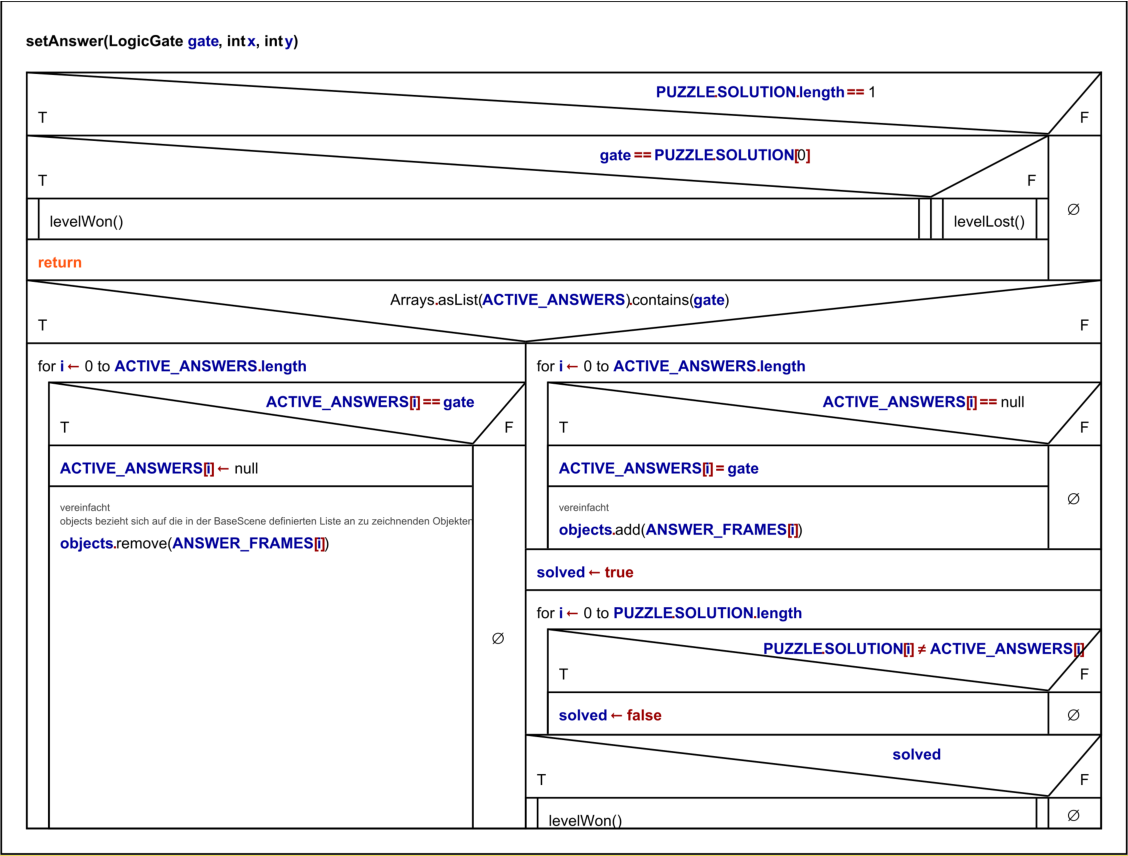
\includegraphics[width=1\textwidth]{bilder/StruktogrammSetAnswer.pdf}
	\caption{Struktogramm der setAnswer-Methode}
	\label{fig:mgsetAnswer}
\end{figure}

\subsubsection{Mathematik}

\begin{sloppypar}
    Für das Minispiel der Fachschaft Mathematik wurde die \texttt{LevelScene} zur \texttt{MathematicsLevelScene} erweitert, um das Zeichnen und Überprüfen der Tangramsteine, sowie das Zeichnen der Silhouette zu ermöglichen.
    Außerdem wurde eine \texttt{TangramPieceObject}-Klasse, welche die Tangramsteine verwaltet, sowie ein \texttt{MathematicsPuzzle}-Enum, das die Silhouette bereitstellt, hinzugefügt.    
\end{sloppypar}

\paragraph{TangramPieceObject} Diese Klasse erweitert das \texttt{BaseObject}.
Dadurch sorgt sie dafür, dass jeder Stein ein Bild besitzt und verschoben, sowie rotiert werden kann.
Sie beinhaltet:

\begin{sloppypar}
    \begin{itemize}
        \item \texttt{SPRITE\_PATH}: Der Pfad zum Bild des Steines.
        \item \texttt{originalWidth, originalHeight}: Die Ausgangsgröße des Steines.
        \item \texttt{rotation}: Die Rotation des Steines.
        \item \texttt{levelScene}: Die \texttt{MathematicsLevelScene}, zu der der Stein gehört.
        \item \texttt{isDragged}: Ein \texttt{boolean}, welcher speichert, ob der Stein gerade gezogen wird.
        \item \texttt{generatePieces()}: Eine statische Methode, die ein Array, welches alle Tangramsteine beinhaltet, zurückgibt.
        \item \texttt{setLevelScene(TangramPieceObject[] pieces, MathematicsLevelScene levelScene)}: Eine statische Prozedur, die bei jedem in \texttt{pieces} gegebenen Tangram-Stein die \texttt{levelScene} festlegt.
        \item \texttt{rotate(double degree)}: Eine Prozedur, die den Stein um den gegebenen Winkel in mathematisch negative Richtung dreht.
        \item \texttt{setRotation(double degree)}: Eine Prozedur, die den Stein so dreht, dass dieser eine Rotation von \texttt{degree} besitzt.
        \item \texttt{update(BaseScene scene)}: Eine Implementierung der \texttt{update}-Prozedur der \texttt{BaseScene}.
            Sie ermöglicht Verschiebung und Drehung des Tangram-Steines.
        \item \texttt{TangramPieceObject(int id)}: Der Konstruktor der Klasse, welcher als \texttt{private} deklariert ist, da immer ein gesamter Satz Tangram-Steine mittels der \texttt{generatePieces}-Methode erstellt werden soll.
            Er lädt das von \texttt{id} abhängige Bild und initialisiert Variablen.
    \end{itemize}
\end{sloppypar}

Die \texttt{update}-Methode ist zur näheren Erklärung im Folgenden dargestellt.

\begin{lstlisting}[caption=update-Methode des TangramPieceObject, label=lst:mggetRandomArray, captionpos=t, language=Java]
public void update(BaseScene scene) {
    // Aktuelle und vorherige Maus-Position abfragen
    Point mousePos = Input.INSTANCE.getMousePosition();
    Point lastMousePos = Input.INSTANCE.getLastMousePosition();
    // Diese *können* (technisch gesehen) null sein
    if(mousePos == null || lastMousePos == null)
        return;

    if (!isDragged && !levelScene.isDragging && isClicked(false)) {
        // Wenn das Objekt angeklickt wird und noch kein Stein
        // gezogen wird, verschieben wir es an oberste Stelle
        // (z-Achse) und beginnen, es zu ziehen
        scene.objects.remove(this);
        scene.objects.add(this);

        isDragged = true;

        // Außerdem teilen wir der levelScene mit,
        // dass jetzt ein Stein gezogen wird
        levelScene.isDragging = true;
    } else if (isDragged && !Input.INSTANCE.getMouseState(MouseEvent.BUTTON1).isDown()) {
        // Wenn die linke Maustaste losgelassen wird,
        // wird das Objekt nicht mehr gezogen,
        isDragged = false;
        // Der levelScene mitgeteilt,
        // dass kein Stein mehr gezogen wird
        levelScene.isDragging = false;
        // Und überprüft, ob das Puzzle gelöst ist
        levelScene.checkPuzzle();
    }

    if (isDragged) {
        // Berechnung der neuen Position
        int newPosX = x + mousePos.x - lastMousePos.x;
        int newPosY = y + mousePos.y - lastMousePos.y;
        // Überprüfung, ob die neue Position innerhalb
        // des Bildschirms liegt
        if (
            newPosX > 0 && newPosX + width < MainWindow.WIDTH &&
            newPosY > 0 && newPosY + height < MainWindow.HEIGHT
        ) {
            // Aktualisierung der Position
            x = newPosX;
            y = newPosY;
        }

        // Rotieren des Objektes, falls 'R' gedrückt wird
        if(
            Input.INSTANCE.getKeyState(KeyEvent.VK_R) ==
            Input.KeyState.PRESSED
        ) {
            rotate(45);
        }
    }
}
\end{lstlisting}

\paragraph{MathematicsPuzzle} Die Implementierung mittels einer Enumeration bietet sich an, da vorgegebene Silhouetten definiert werden, die nicht verändert oder durch weitere ergänzt werden können.
Sie beinhaltet:

\begin{sloppypar}
    \begin{itemize}
        \item \texttt{PUZZLES}: Ein statisches, zweidimensionales \texttt{MathematicsPuzzle}-Array, welches für jedes Level die zugehörigen Enum-Konstanten speichert.
        \item \texttt{SPRITE}: Ein \texttt{java.awt.Image}, das das zum Puzzle gehörende Bild speichert.
        \item \texttt{MARGIN\_OF\_ERROR}: Die prozentuale Abweichung der bedeckten Fläche, sodass eine Belegung trotzdem als Lösung gilt.
        \item \texttt{SOLUTIONS}: Ein dreidimensionales \texttt{double}-Array, welches für jede Lösung (erste Dimension), für jeden Tangram-Stein (zweite Dimension) die X-Position, Y-Position und Rotation (dritte Dimension) speichert.
            Dabei werden erstere als relative Position gespeichert, also als \texttt{double} zwischen $0$ und $1$, der angibt, bei wie viel Prozent der Gesamtbreite beziehungsweise Gesamthöhe sich der Stein befindet.
            Eine Besonderheit stellt der Ausgangszustand, welcher ebenfalls als ein Puzzle gespeichert wird, bei dem alle Steine vorgegeben sind, dar.
            Dieser speichert zusätzlich noch die Breite und die Höhe der Steine, um diese entsprechend zurückzusetzten.
            Wichtig ist, dass diese Lösungen nur zum Vorgeben der Tangramsteine verwendet werden und nicht zur Überprüfung einer Belegung dieser.
            Dadurch ist es auch nicht unbedingt notwendig mehrere Lösungen pro Puzzle zu definieren, jedoch entsteht dadurch mehr Variabilität.
        \item \texttt{AMOUNT\_OF\_GIVEN\_PIECES}: Die Anzahl an bereits platzierten Steinen.
        \item \texttt{ANSWERS}: Ein \texttt{LogicGate}-Array, das die zur Auswahl stehenden Antwortmöglichkeiten beinhaltet.
        \item \texttt{getPuzzle(int level)}: Eine Methode, welche eine zufällige Enum-Konstante basierend auf dem gegebenen level, mittels der \texttt{java.util.Random}-Klasse zurückgibt.
        \item \texttt{isSolutionValid(int x, int y, int width)}: Eine Methode, die berechnet, wie viele Pixel der Silhouette von Tangramsteinen verdeckt sind und wie viele Pixel die Silhouette insgesamt enthält.
            Dadurch wird dann ermittelt, wie viel Prozent der Silhoutte verdeckt sind und $p\% < 1-MARGIN\_OF\_ERROR$ zurückgegeben.
        \item \texttt{setGivenPieces(TangramPieceObject[] pieces, int x, int y, int width, int height)}: Eine Prozedur, die die richtige Position und Rotation zufällig aus \texttt{pieces} ausgewählter Tangramsteine vorgibt.
        \item \texttt{reset(TangramPieceObject[] pieces, int x, int y, int size, int px, int py, int pwidth, int pheight)}: Eine Prozedur, welche die Steine mittels \texttt{setGivenPieces} in den Ausgangszustand zurücksetzt und neu für das Puzzle vorgibt.
        \item \texttt{MathematicsPuzzle(String path, int amountOfGivenPieces, double[][][] solutions)}: Der Konstruktor der Klasse, welcher nur von der Klasse selbst bei der Initialisierung der Konstanten aufgerufen wird.
            Er initialisiert die Variablen mit den durch die Parameter gegebenen Werten.
    \end{itemize}
\end{sloppypar}

Die \texttt{setGivenPieces}-Methode ist zur näheren Erklärung im Folgenden dargestellt.
Da sie teilweise stark der im Programmcode \ref{lst:mggetRandomArray} abgebildeten Methode ähnelt wurde sie verkürzt dargestellt.

\begin{lstlisting}[caption=update-Methode des TangramPieceObject, label=lst:mggetRandomArray, captionpos=t, language=Java]
private void setGivenPieces(
    TangramPieceObject[] pieces, int x, int y, int width, int height
) {
    // Generierung der zufälligen Indizes der vorzugebenden Steine
    int[] idx = new int[AMOUNT_OF_GIVEN_PIECES];
    
    [ausgelassen]

    // Festlegen einer Lösung des Puzzles
    int rSolution = new Random().nextInt(SOLUTIONS.length);
    // Positionierung der Steine
    for(int i : idx) {
        // Rotation wird als erstes geändert, da sich dadurch
        // die Größe und somit die Position des Steines ändern kann.
        pieces[i].setRotation(SOLUTIONS[rSolution][i][2]);
        pieces[i].x = (int) (x + SOLUTIONS[rSolution][i][0]*width);
        pieces[i].y = (int) (y + SOLUTIONS[rSolution][i][1]*height);

        // Höhe und Breite der Steine zurücksetzten,
        // falls es sich beim Puzzle um den Ausgangszustand handelt
        if(this == P_INIT) {
            pieces[i].width =
            (int) (SOLUTIONS[rSolution][i][3]*width);
            pieces[i].height =
            (int) (SOLUTIONS[rSolution][i][4]*height);
            pieces[i].originalWidth = pieces[i].width;
            pieces[i].originalHeight = pieces[i].height;
        }
    }
}
\end{lstlisting}

\paragraph{MathematicsLevelScene} Eine erweiterung der \texttt{LevelScene}, welche die grundlegenden Methoden des Mathematik-Minispieles implementiert.
Sie beinhaltet:

\begin{sloppypar}
    \begin{itemize}
        \item \texttt{PIECES}: Ein \texttt{TangramPieceObject}-Array, welches die Tangramsteine des Levels speichert.
        \item \texttt{PUZZLE}: Das \texttt{MathematicsPuzzle} des Levels.
        \item \texttt{PUZZLE\_X}: Die X-Position der Silhouette.
        \item \texttt{PUZZLE\_Y}: Die Y-Position der Silhouette.
        \item \texttt{PUZZLE\_WIDTH}: Die Breite der Silhouette.
        \item \texttt{PUZZLE\_HEIGHT}: Die Höhe der Silhouette.
        \item \texttt{isDragging}: Ein \texttt{boolean}, der speichert, ob gerade ein Tangramstein gezogen wird.
            Dadurch wird verhindert, dass mehrere Steine gleichzeitig gezogen werden.
        \item \texttt{reset()}: Eine Methode, die die \texttt{reset}-Methode der \texttt{LevelScene} implementiert, indem sie eine neu generierte \texttt{MathematicsLevelScene} zurückgibt.
        \item \texttt{checkPuzzle()}: Eine Prozedur, die mittels der \texttt{isSolutionValid}-Methode des \texttt{PUZZLE} überprüft, ob das Level gelöst wurde und in diesem Fall das Level beendet.
        \item \texttt{MathematicsLevelScene(int level)}: Der Konstruktor der Klasse, welcher alle Variablen initialisiet und die Steine, sowie die Silhouette platziert.
    \end{itemize}
\end{sloppypar}

\subsubsection{Chemie}

\begin{sloppypar}
    Für das Minispiel der Fachschaft Chemie wurde die \texttt{LevelScene} zur \texttt{ChemieLevelScene} erweitert.
    Die gesamte Spiellogik ist auf zwei Klassen aufgeteilt: \texttt{ChemieGameObject}, welches den Timer sowie die Spiellogik verwaltet, und \texttt{Reagenzglas}, welches ein einzelnes Reagenzglas als \texttt{BaseObject} repräsentiert.
\end{sloppypar}

\paragraph{Reagenzglas}
Eine Erweiterung von \texttt{BaseObject}, die ein einzelnes Reagenzglas darstellt.
Die Klasse beinhaltet:

\begin{sloppypar}
    \begin{itemize}
        \item \texttt{MAX\_KAPAZITAET}, \texttt{GLAS\_BREITE}, \texttt{GLAS\_HOEHE}: Statische Konstanten, die die maximale Anzahl an Blöcken, sowie die Darstellungsgröße eines Reagenzglases definieren.
        \item \texttt{blockBilder}: Eine \texttt{Map<String, Image>}, die Farbnamen auf die zugehörigen Block-Bilder abbildet.
        \item \texttt{blockHinzufuegen(String farbe)}: Fügt einen Block der gegebenen Farbe oben ins Reagenzglas ein, sofern es nicht voll ist.
        \item \texttt{oberstenBlockEntfernen()}: Entfernt den obersten Block und gibt seine Farbe zurück.
        \item \texttt{oberstenBlockAnschauen()}: Gibt die Farbe des obersten Blocks zurück, \textbf{ohne} ihn zu entfernen.
        \item \texttt{istLeer()}, \texttt{istVoll()}: Abfragen des Füllzustands.
        \item \texttt{istGeloest()}: Gibt \texttt{true} zurück, wenn das Glas vollständig mit Blöcken einer einzigen Farbe gefüllt ist.
        \item \texttt{kannAblegen(String farbe)}: Gibt \texttt{true} zurück, wenn ein Block der gegebenen Farbe abgelegt werden darf, d.h. das Glas nicht voll ist und entweder leer ist oder der oberste Block die gleiche Farbe hat.
        \item \texttt{setAusgewaehlt(boolean)}: Verschiebt das Reagenzglas um 10 Pixel nach oben bzw. unten und aktualisiert den Auswahlzustand.
        \item \texttt{draw(Graphics2D g)}: Zeichnet das Reagenzglasbild via \texttt{super.draw(g)} und anschließend die enthaltenen Farbblöcke.
    \end{itemize}
\end{sloppypar}

\textbf{Beispielcode aus Reagenzglas}
\begin{lstlisting}[caption=istGeloest-Methode, label=lst:mgistgeloest, captionpos=t, language=Java]
public boolean istGeloest() {
    // Glas muss vollstaendig gefuellt sein
    if (bloecke.size() != MAX_KAPAZITAET) return false;
    // Alle Bloecke muessen die gleiche Farbe haben
    String f = bloecke.get(0);
    for (String b : bloecke) if (!b.equals(f)) return false;
    return true;
}
\end{lstlisting}

\paragraph{ChemieGameObject}
Eine Erweiterung von \texttt{BaseObject}, die das gesamte Chemie-Minigame verwaltet.

Sie beinhaltet:
\begin{sloppypar}
    \begin{itemize}
        \item \texttt{blockBilder}: Eine \texttt{Map<String, Image>}, die Farbnamen auf die zugehörigen Block-Bilder abbildet und an alle \texttt{Reagenzglas}-Objekte weitergereicht wird.
        \item \texttt{glaeser}: Eine \texttt{List<Reagenzglas>}, die alle Reagenzgläser des aktuellen Levels enthält.
        \item \texttt{ausgewaehltesGlas}: Der Index des aktuell ausgewählten Glases, oder \texttt{-1} wenn keines ausgewählt ist.
        \item \texttt{verbleibendeSekunden}: Die verbleibende Zeit in Sekunden.
        \item \texttt{levelErstellen()}: Initialisiert die Reagenzgläser mit zufällig verteilten Farbblöcken abhängig vom Level sowie zwei leeren Puffergläsern und berechnet deren Positionen.
        \item \texttt{umschuetten(int von, int nach)}: Schüttet alle aufeinanderfolgenden Blöcke gleicher Farbe vom Quell- ins Zielglas um, sofern dies möglich ist.
        \item \texttt{istGewonnen()}: Gibt \texttt{true} zurück, wenn alle nicht-leeren Gläser gelöst sind.
        \item \texttt{update(BaseScene)}: Aktualisiert den Timer, ruft bei Ablauf \texttt{levelLost()} auf und erkennt Klicks auf Reagenzgläser mittels \texttt{isClicked()}.
        \item \texttt{draw(Graphics2D)}: Zeichnet Titel, Hinweistext und Timer und delegiert das Zeichnen der Gläser an die jeweiligen \texttt{Reagenzglas}-Objekte.
    \end{itemize}
\end{sloppypar}

Die \texttt{umschuetten}-Methode ist zur näheren Erklärung im Folgenden dargestellt.

\textbf{Beispielcode aus ChemieGameObject}
\begin{lstlisting}[caption=umschuetten-Methode, label=lst:mgumschuetten, captionpos=t, language=Java]
private void umschuetten(int von, int nach) {
    Reagenzglas v = glaeser.get(von);
    Reagenzglas n = glaeser.get(nach);
    // Farbe des obersten Blocks im Quellglas
    String farbe = v.oberstenBlockAnschauen();
    // Abbruch, wenn Quellglas leer oder Ablegen nicht moeglich
    if (farbe == null || !n.kannAblegen(farbe)) return;
    // Alle aufeinanderfolgenden Bloecke gleicher Farbe umschuetten
    while (v.oberstenBlockAnschauen() != null
            && v.oberstenBlockAnschauen().equals(farbe)
            && n.kannAblegen(farbe))
        n.blockHinzufuegen(v.oberstenBlockEntfernen());
}
\end{lstlisting}

\paragraph{ChemieLevelScene}
Eine Erweiterung der \texttt{LevelScene}, welche das \texttt{ChemieGameObject} zur \texttt{objects}-Liste hinzufügt.

Sie beinhaltet:
\begin{sloppypar}
    \begin{itemize}
        \item \texttt{reset()}: Gibt eine neu erstellte \texttt{ChemieLevelScene} zurück.
        \item \texttt{ChemieLevelScene(int level)}: Der Konstruktor, der das Hintergrundbild sowie ein neues \texttt{ChemieGameObject} zur Szene hinzufügt.
    \end{itemize}
\end{sloppypar}

\subsubsection{Physik}

\begin{sloppypar}
    Für das Minispiel der Fachschaft Physik wurde die \texttt{LevelScene} zur \texttt{PhysikLevelScene} erweitert.
    Die gesamte Spiellogik ist im \texttt{PhysikGameObject} gekapselt, welches die Physik-Simulation, die Kraftpfeil-Eingabe sowie den Simulate-Button verwaltet.
\end{sloppypar}

\paragraph{PhysikGameObject}
Eine Erweiterung von \texttt{BaseObject}, die das gesamte Physik-Minigame verwaltet.
Das Spiel läuft in drei Phasen ab: \texttt{PHASE\_VORBEREITUNG}, in der der Spieler einen Kraftpfeil vom Ball wegzieht, \texttt{PHASE\_SIMULATION}, in der der Ball unter Einfluss der Beschleunigungen fliegt, und \texttt{PHASE\_ERGEBNIS}, die nach dem Treffem oder Verfehlen bzw der Kollison mit Boden oder Wand eintritt.

Die Klasse beinhaltet:
\begin{sloppypar}
    \begin{itemize}
        \item \texttt{simulateButton}: Ein \texttt{ButtonObject}, das die Simulation startet und nur in \texttt{PHASE\_VORBEREITUNG} angezeigt und aktualisiert wird.
        \item \texttt{basisBeschleunigungen}: Ein zweidimensionales \texttt{double}-Array, das die levelspezifischen Beschleunigungen (z.B. Gewichtskraft, Drift) speichert.
        \item \texttt{kraftRichtung}: Ein \texttt{String} (\texttt{"RIGHT"} oder \texttt{"UP"}), der die erlaubte Zugrichtung des Kraftpfeils vorgibt.
        \item \texttt{wand}: Ein \texttt{int}-Array \texttt{\{x, y, breite, hoehe\}}, das die Position der Wand in Level 3 beschreibt, oder \texttt{null} in den anderen Levels.
        \item \texttt{ziel}: Ein \texttt{double}-Array \texttt{\{x, y, breite, hoehe\}}, das die Position des Ziels beschreibt.
        \item \texttt{levelInitialisieren()}: Setzt Ball, Geschwindigkeit und Spielerkraft zurück und konfiguriert die levelspezifischen Parameter.
        \item \texttt{simulationStarten()}: Übernimmt die Spielerkraft als Startgeschwindigkeit und wechselt in \texttt{PHASE\_SIMULATION}.
        \item \texttt{ballBewegen()}: Wendet alle Basisbeschleunigungen auf die Geschwindigkeit an, bewegt den Ball und prüft Kollisionen mit Rand, Wand und Ziel.
        \item \texttt{simulationStoppen(boolean treffer)}: Wechselt in \texttt{PHASE\_ERGEBNIS} und ruft \texttt{levelWon()} bzw. \texttt{levelLost()} auf.
        \item \texttt{update(BaseScene)}: Verarbeitet Maus-Drag zur Kraftpfeil-Eingabe, delegiert Button-Klicks an \texttt{simulateButton} und führt die Simulation schrittweise aus.
        \item \texttt{draw(Graphics2D)}: Zeichnet Titel, Hinweistext, Ziel und die Kraftpfeile.
    \end{itemize}
\end{sloppypar}

\textbf{Beispielcode aus PhysikGameObject} \\
Im folgenden Codeausschnitt werden die drei Level (0, 1, 2 bzw. 1, 2, 3) von einander durch verschiedene Eigenschaften unterschieden.
\begin{lstlisting}[caption=Case Switch für die Level, label=lst:mgSwitch(level), captionpos=t, language=Java]
// Level-spezifische Konfiguration
        switch (level) {
                        case 0:
                            // Nur Schwerkraft nach unten, Spieler schießt nach rechts
                            basisBeschleunigungen = new double[][]{{0, GRAVITY}};
                            // Spieler*in kann Kraftpfeil nur nach rechts ziehen
                            kraftRichtung = "RIGHT";
                            wand = null;
                        break;
                        case 1:
                            // Schwerkraft + leichter Drift nach links
                            basisBeschleunigungen = new double[][]{{0, GRAVITY}, {-0.05, 0}};
                            // Spieler*in kann Kraftpfeil nur nach rechts ziehen
                            kraftRichtung = "RIGHT";
                            wand = null;
                        break;
                        default:
                            // Schwerkraft + starker Drift nach rechts + Wand in der Mitte
                            basisBeschleunigungen = new double[][]{{0, GRAVITY}, {0.12, 0}};
                            // Spieler*in kann Kraftpfeil nur nach oben ziehen
                            kraftRichtung = "UP";
                            wand = new int[]{
                                             BREITE / 4,
                                             HOEHE / 3,
                                             30,
                                             133
                            };
                        break;
                        }
    }
\end{lstlisting}

Im folgenden Codeausschnitt wird die Bewegung des Balles, basierend auf den Basis- und Spielerkräften ausgeführt, sowie die Gewinnbedingungen geprüft.
\begin{lstlisting}[caption=ballBewegen-Methode, label=lst:mgballbewegen, captionpos=t, language=Java]
private void ballBewegen() {
    // Alle Basisbeschleunigungen auf Geschwindigkeit addieren
    for (double[] a : basisBeschleunigungen) {
        velX += a[0];
        velY += a[1];
    }
    // Geschwindigkeit auf Position addieren
    ballX += velX;
    ballY += velY;
    // Fensterrand getroffen -> verloren
    if (ballX <= 0 || ballX + BALL_GROESSE >= BREITE
            || ballY <= 0 || ballY + BALL_GROESSE >= HOEHE) {
        simulationStoppen(false);
        return;
    }
    // Wand getroffen (Level 3) -> verloren
    if (wand != null && new Rectangle((int) ballX, (int) ballY,
            BALL_GROESSE, BALL_GROESSE)
            .intersects(new Rectangle(wand[0], wand[1], wand[2], wand[3]))) {
        simulationStoppen(false);
        return;
    }
    // Ziel getroffen -> gewonnen
    if (new Rectangle((int) ballX, (int) ballY, BALL_GROESSE, BALL_GROESSE)
            .intersects(new Rectangle(
                    (int) ziel[0], (int) ziel[1],
                    (int) ziel[2], (int) ziel[3]))) {
        simulationStoppen(true);
    }
}
\end{lstlisting}

\paragraph{PhysikLevelScene}
Eine Erweiterung der \texttt{LevelScene}, welche das \texttt{PhysikGameObject} zur \texttt{objects}-Liste hinzufügt.

Sie beinhaltet:
\begin{sloppypar}
    \begin{itemize}
        \item \texttt{reset()}: Gibt eine neu erstellte \texttt{PhysikLevelScene} zurück.
        \item \texttt{PhysikLevelScene(int level)}: Der Konstruktor, der das Hintergrundbild sowie ein neues \texttt{PhysikGameObject} zur Szene hinzufügt.
    \end{itemize}
\end{sloppypar}

\subsubsection{Biologie}

\begin{sloppypar}
    Für das Minispiel der Fachschaft Biologie wurde die \texttt{LevelScene} zur \texttt{BiologieLevelScene} erweitert, hier findet sich die Spiellogic.
    Die Klasse \texttt{BiologyData} lädt alle Pflanzenbilder und speichert sie levelweise in den \texttt{static final}-Arrays: \texttt{LEVEL\_1\_PLANTS}, \texttt{LEVEL\_2\_PLANTS} und \texttt{LEVEL\_3\_PLANTS}.
    Die Klasse \texttt{BiologyPlant} speichert das Bild und den Namen einer Pflanze.
    \texttt{BiologyLabelObject} erweitert das BaseObject. Es zeichnet die Label und setzt den Status selected oder nicht selected.
\end{sloppypar}

\paragraph{BiologyLevelScene}
Eine Erweiterung von \texttt{BaseScene}, die das gesamte Biologie-Minigame verwaltet.
Der Spieler sieht vier zufällig ausgewählte Pflanzenbilder und muss diesen die richtigen Namen zuordnen, indem er Labels anklickt und auf die passenden Bilder platziert.

Die Klasse beinhaltet:
\begin{sloppypar}
    \begin{itemize}
        \item \texttt{selectedLabel}: Das aktuell ausgewählte \texttt{BiologyLabelObject}, oder \texttt{null}, falls keines ausgewählt ist.
        \item \texttt{imagePlaceholders}: Ein Array aus vier \texttt{BaseObject}-Instanzen, die die angezeigten Pflanzenbilder repräsentieren.
        \item \texttt{chosen}: Eine \texttt{List<BiologyPlant>} mit den vier zufällig gewählten Pflanzen des aktuellen Durchlaufs.
        \item \texttt{getLabelAtSlot(int slot)}: Gibt das \texttt{BiologyLabelObject} zurück, das aktuell einem bestimmten Bildslot zugeordnet ist, oder \texttt{null}, falls keines platziert wurde.
        \item \texttt{reset()}: Erstellt eine neue \texttt{BiologyLevelScene} mit demselben Level und setzt damit das Spiel vollständig zurück.
        \item \texttt{update()}: Verarbeitet Klick-Interaktionen: wählt ein Label aus, hebt die Auswahl auf oder platziert das ausgewählte Label auf einem Bildslot. Nach jeder Platzierung wird geprüft, ob alle Slots belegt sind, und bei Vollständigkeit \texttt{checkWin()} aufgerufen.
        \item \texttt{checkWin()}: Prüft für jeden der vier Bildslots, ob das dort platzierte Label mit dem Namen der zugehörigen Pflanze übereinstimmt.
        \item \texttt{allPlaced()}: Gibt \texttt{true} zurück, wenn alle vier Bildslots mit einem Label belegt sind.
    \end{itemize}
\end{sloppypar}

Im Konstruktor wird abhängig vom \texttt{LEVEL}-Wert der passende Pflanzen-Pool (\texttt{LEVEL\_1\_PLANTS}, \texttt{LEVEL\_2\_PLANTS} oder \texttt{LEVEL\_3\_PLANTS}) geladen. Daraus werden vier Pflanzen zufällig gezogen und deren Bilder auf Slotgröße skaliert und zugeschnitten.
Die Label-Liste enthält stets die vier richtigen Namen sowie je nach Schwierigkeitsgrad ein (Level 2) oder zwei (Level 3) zusätzliche falsche Labels, die ebenfalls zufällig gemischt werden.

Dieser Beispielcode zeigt der Verarbeitung der Pflanzenbilder für das Minigame.
Jedes Pflanzenbild wird dabei proportional skaliert und mittig zugeschnitten, sodass es exakt in den vorgegebenen Slot passt, bevor es als \texttt{BaseObject} zur Szene hinzugefügt wird.

\begin{lstlisting}[caption=Skalierung Pflanzenbilder, label=lst:mgBildskalierung, captionpos=t, language=Java]
// Originalbild der gewaehlten Pflanze laden
BufferedImage original = (BufferedImage) chosen.get(i).image;

// Skalierungsfaktor berechnen: Bild soll den Slot vollstaendig ausfuellen
double scale = Math.max((double) slotW / original.getWidth(),
                        (double) slotH / original.getHeight());
int scaledW = (int) (original.getWidth() * scale);
int scaledH = (int) (original.getHeight() * scale);

// Neues Bild in der skalierten Groesse erstellen
BufferedImage scaled = new BufferedImage(scaledW, scaledH,
                                         BufferedImage.TYPE_INT_RGB);
Graphics2D g2d = scaled.createGraphics();

// Originalbild in die neue skalierte Groesse zeichnen
g2d.drawImage(original, 0, 0, scaledW, scaledH, null);


// Grafikkontext freigeben, um Ressourcen zu vermeiden
g2d.dispose();

// Bild mittig auf Slotgroesse zuschneiden (Center-Crop)
int cropX = Math.max(0, (scaledW - slotW) / 2);
int cropY = Math.max(0, (scaledH - slotH) / 2);
int cropW = Math.min(slotW, scaledW);
int cropH = Math.min(slotH, scaledH);
Image cropped = scaled.getSubimage(cropX, cropY, cropW, cropH);

// Zugeschnittenes Bild als BaseObjekt hinzufuegen
BaseObject plantImage = new BaseObject(cropped,
                                       imageX[i] * PIXEL_SCALE,
                                       imageY[i] * PIXEL_SCALE);
plantImage.width = cropW * PIXEL_SCALE;
plantImage.height = cropH * PIXEL_SCALE;

// Objekt im Slot-Array speichern (fuer spaetere Klick-Erkennung)
// und der Szene hinzufuegen, damit es gezeichnet wird
imagePlaceholders[i] = plantImage;
objects.add(plantImage);
\end{lstlisting}

Dieser Codeausschnitt zeigt die Klick-Interaktionslogik des Spiels:
Ein Label wird ausgewählt, auf einen Bildslot platziert – wobei ein bereits vorhandenes Label automatisch zurück in die Label-Leiste wandert – und, wenn allen Bildern ein Label zugeordnet sind wird geprüft, ob die Zuordnung richtig ist.

\begin{lstlisting}[caption=Label Zuordnung und Gewinnbedingungen prüfen, label=lst:mgLabelzuordnung, captionpos=t, language=Java]
 public void update() {
        super.update();

// Ist kein Label ausgewaehlt, auf Klick eines Labels pruefen
if (selectedLabel == null) {
    for (BaseObject obj : objects) {
        if (obj instanceof BiologyLabelObject label) {
            if (label.isClicked()) {
                // Label als ausgewaehlt markieren und merken
                selectedLabel = label;
                label.selected = true;
            }
        }
    }
} else {
    // Klick auf das bereits ausgewaehlte Label hebt Auswahl wieder auf
    if (selectedLabel.isClicked()) {
        selectedLabel.selected = false;
        selectedLabel = null;
        return;
    }

    // Pruefen, ob eines der vier Bildslots angeklickt wurde
    for (int i = 0; i < 4; i++) {
        if (imagePlaceholders[i].isClicked()) {

            // Falls Slot bereits belegt, vorhandenes Label
            // zurueck in die Label-Leiste verschieben
            BiologyLabelObject existing = getLabelAtSlot(i);
            if (existing != null) {
                // Index des bestehenden Labels unter allen Labels ermitteln,
                // um seine urspruengliche Position zu berechnen
                int idx = 0;
                for (BaseObject obj : objects) {
                    if (obj instanceof BiologyLabelObject lbl) {
                        if (lbl == existing) break;
                        idx++;
                    }
                }
                // Label an seine urspruengliche Position
                existing.x = (10 + (idx % 3) * 55) * PIXEL_SCALE;
                existing.y = (105 + (idx / 3) * 16) * PIXEL_SCALE;
            }

            // Ausgewaehltes Label auf den angeklickten Bildslot platzieren
            selectedLabel.x = imageX[i] * PIXEL_SCALE;
            selectedLabel.y = 71 * PIXEL_SCALE;
            selectedLabel.selected = false;
            selectedLabel = null;

            // Wenn alle vier Slots belegt sind, Gewinnpruefung starten
            if (allPlaced()) {
                if (checkWin()) {
                    levelWon();
                } else {
                    levelLost();
                }
            }
        }
    }
}
\end{lstlisting}

\paragraph{BiologyLabelObject}
Eine Erweiterung von \texttt{BaseObject}, die ein anklickbares, beschriftetes Label darstellt, das der Spieler per Klick auswählen und auf einem Bildslot platzieren kann.

Die Klasse beinhaltet:
\begin{sloppypar}
    \begin{itemize}
        \item \texttt{name}: Ein \texttt{String}, der den angezeigten Pflanzennamen enthält.
        \item \texttt{selected}: Ein \texttt{boolean}, der angibt, ob das Label aktuell vom Spieler ausgewählt ist.
        \item \texttt{draw(Graphics2D g)}: Zeichnet das Label als gefülltes Rechteck mit zentriertem Text. Der Hintergrund wird hellgrau dargestellt, wenn das Label ausgewählt ist, andernfalls weiß. Der Pflanzenname wird leicht eingerückt und vertikal zentriert in der Box gezeichnet.
    \end{itemize}
\end{sloppypar}

\begin{lstlisting}[caption=Zeichen des Labels, abhängig vom Zustand, label=lst:mgDrawLabel, captionpos=t, language=Java]
    public void draw(Graphics2D g) {
    //falls das Label selected ist, Hintergrund LIGHT_GRAY
        if (selected) {
            g.setColor(Color.LIGHT_GRAY);
        } else {
        //sonst WHITE
            g.setColor(Color.WHITE);
        }
        //Rechteck mit schwarzen Linien zeichnen
        g.fillRect(x, y, width, height);
        g.setColor(Color.BLACK);
        //Pflanzennamen zentriert plazieren
        g.drawString(name, x + 5, y + (height / 2)+3 );
    }
\end{lstlisting}



\section{Item- und Charakterdesign}

Um den Spieler, die Lehrerinnen und Lehrer, sowie die Items in das Programm einzubinden, haben wir diese als Spiel-Objekte, also als Unterklassen von \texttt{BaseObject} implementiert, da sie so gut mit den in der Lösungsidee beschriebenen Eigenschaften versehen werden konnten. Dafür haben wir die Klassen \texttt{PlayerObject}, \texttt{LehrerObject} und \texttt{ItemType} umgesetzt.

\subsection{\texttt{PlayerObject}}
Das \texttt{PlayerObject} erweitert das \texttt{BaseObject} und übernimmt so wichtige Eigenschaften. Dieses beinhaltet die Funktionalität zur Gestaltung der Figur, des Kampfes und des Inventares. Hierbei ist das Inventar eine Liste. Beim gewinnen eines Minispiels wird, wie oben erwähnt, ein Item dem Array hinzugefügt.

Die Klasse stellt außerdem eine Singleton-Instanz von sich bereit, die
Spielfigur wird also genau einmal instantiiert.

In ihrer \texttt{update}-Methode überprüft die Spielfigur mithilfe \texttt{BaseObject.isClicked}, ob sie angeklickt wurde. Ist dies der Fall, wird eine neue Instanz der in Kürze beschriebenen \texttt{InventarScene} auf den Szenenstapel gepushed.

\begin{lstlisting}[caption=PlayerObject, label=programm:playerobject, captionpos=t, language=Java]
public class PlayerObject extends BaseObject{
	
	//Anlegen einer Reihung "Inventar", in welchem die Items, auf die der Spieler zugreifen kann, gespeichert werden
	public final List<ItemType> inventar = new ArrayList<>();
	
	[...]
	
	/**
	* Singleton-Instanz
	*/
	public static final PlayerObject INSTANCE = new PlayerObject();
	
	
	/**
	* Privater Konstruktor, der nur für {@link #INSTANCE} verwendet wird
	*/
	private PlayerObject() {
		// Vorläufig ohne Bild initialisieren
		super(null);
		
		// Vorlage laden und Größe bestimmen
		Image baseSprite = Images.get("/assets/characters/PlayerBase.png");
		width = baseSprite.getWidth(null) * PIXEL_SCALE;
		height = baseSprite.getHeight(null) * PIXEL_SCALE;
		
		[...]
	}
	
	//Funktion zum Festlegen einer zufälligen x-Koordinate für die Spieler-Figur
	public static int GetRandomX(){
		Random r = new Random();
		int min = 35;
		int max = 790;
		return r.nextInt((max - min) + 1) + min;
	}
	
	[...]
	
	
	@Override
	public void update(BaseScene scene) {
		// Inventar öffnen, wenn die Figur angeklickt wird
		if(isClicked())
		SceneStack.INSTANCE.push(new InventarScene());
	}
	
}

\end{lstlisting}


\subsubsection{InventarScene}

Die Inventar-Szene stellt die Items dar, die im Besitz der Spielfigur sind.
Dabei ist jedoch das einzige tatsächliche Spiel-Objekt, welches sie beinhaltet,
der \glqq{}X\grqq{}-Knopf, durch dessen Klicken sie sich wieder vom Szenenstapel
entfernt. Das Anzeigen der Items wird über das Erweitern von \texttt{BaseObject.draw}
gelöst.

\begin{lstlisting}[caption=InventarScene, label=programm:inventarscene, captionpos=t, language=Java]
public class InventarScene extends BaseScene {
	
	/**
	* X-Koordinate der linken Seite
	*/
	private static final int iLeft = (int)(WIDTH * 0.03);
	/**
	* Y-Koordinate der oberen Seite
	*/
	private static final int iTop = (int)(HEIGHT * 0.03);
	/**
	* Breite des Inventars
	*/
	private static final int iWidth = WIDTH - 2 * iLeft;
	/**
	* Höhe des Inventars
	*/
	private static final int iHeight = (int)(HEIGHT * 0.3);
	/**
	* Abstand zwischen Items
	*/
	private static final int iPadding = (int)(WIDTH * 0.025);
	
	public InventarScene() {
		// Button zum Schließen
		ButtonObject exit = new ButtonObject (
		Images.get("/assets/minigames/general/button_exit.png"),
			SceneStack.INSTANCE::pop
		);
		
		exit.x = iLeft + iWidth - iPadding - exit.sprite.getWidth(null) * PIXEL_SCALE;
		exit.y = iTop + (iHeight / 2) - (exit.sprite.getHeight(null) * PIXEL_SCALE )/2;
		objects.add(exit);
	}
	
	@Override
	public void draw(Graphics2D g) {
		// Hintergrund
		g.setColor(new Color(0x9A6B9C));
		g.fillRect(iLeft, iTop, iWidth, iHeight);
		
		// Für Text
		g.setColor(Color.WHITE);
		g.setFont(Draw.FONT_TITLE.deriveFont(20f));
		
		// Items mit Beschriftung zeichnen
		int x = iLeft + iPadding;
		for (int i = 0; i < PlayerObject.INSTANCE.inventar.size(); i++) {
			// Item abfragen
			ItemType item = PlayerObject.INSTANCE.inventar.get(i);
			
			// Sprite zeichnen
			int y = iTop + ((int) (HEIGHT * 0.05));
			g.drawImage(item.SPRITE, x, y, item.SPRITE.getWidth(null) * PIXEL_SCALE, item.SPRITE.getHeight(null) * PIXEL_SCALE, null);
			
			// Text zeichnen
			Draw.drawTextCentered(g, item.NAME, x + item.SPRITE.getWidth(null) * PIXEL_SCALE / 2, y + item.SPRITE.getHeight(null) * PIXEL_SCALE + 32);
			
			x += item.SPRITE.getWidth(null) * PIXEL_SCALE + iPadding;
		}
		
		// Objekte
		super.draw(g);
	}
	
}

\end{lstlisting}

\subsection{LehrerObject}
Das \texttt{LehrerObject} ist ebenfalls eine Erweiterung des \texttt{BaseObject} und fügt die in der Lösungsidee besprochenen Eigenschaften von Schwierigkeit, Lebenspunkten, Fachschaft und eine Liste aus im Kampf zu verwendenen Items zu. Diese sind hier das Integer Level und hp (Healthpoints), der String Fachschaft und das Array Lehrer-Items. Diese werden dann zusammen mit den Parametern aus dem BaseObjekt im darauffolgenden Constructor initialisiert. Darauffolgend sind wieder die Funktionen für den Kampf.
\\
\begin{lstlisting}[caption=LehrerObject, label=programm:lehrerobject, captionpos=t, language=Java]
    public class LehrerObject extends BaseObject{

    public final int LEVEL;
    public int hp;
    public final String FACHSCHAFT;
    public final List<ItemType> lehrer_items;

    public LehrerObject(Image sprite, int x, int y, String FACHSCHAFT, int hp, int LEVEL, List<ItemType> lehrer_items) {
        super(sprite, x, y);
        this.LEVEL = LEVEL;
        this.hp = hp;
        this.FACHSCHAFT = FACHSCHAFT;
        this.lehrer_items = lehrer_items;
    }

    public void verteidigung(int level) {
        // Es wird zufällig ausgewählt, ob ein Item gewählt wird (und welches), oder ob der Lehrer nichts macht.
        Random rand = new Random();
        int move = rand.nextInt(5);
        int schaden;
        ItemType item_lehrer;

        if (move == 0) {
            schaden = level;
            item_lehrer = null;
        }
        else {
            item_lehrer = lehrer_items.get(move - 1);
            schaden = level - item_lehrer.LEVEL;
            if (schaden <= 0) {
                schaden = 0;
            }

        }

        hp -= schaden;

    }
    
    public void angriff() {
        Random rand = new Random();
        int move = rand.nextInt(4);
        int level;
        ItemType item_lehrer;
        
        item_lehrer = lehrer_items.get(move);
        level = item_lehrer.LEVEL;
        
        PlayerObject.INSTANCE.verteidigung(level);
    }

    @Override
    public void update(BaseScene scene) {
    }
}
\end{lstlisting}

\subsection{ItemType}
Die Items sind in der Form von im Glossar erklärten Enums gespeichert. Jedes Enum hat einen Namen und eine am Anfang festgelegte Anzahl von Parametern und deren Datentypen: der String NAME für den Namen des Items, das Image SPRITE für die Bilddatei und den Integer LEVEL für die Stärke des Items. 

\begin{lstlisting}[caption=ItemType, label=programm:itemtype, captionpos=t, language=Java]
    public enum ItemType {
    ATOM("Atom", "/assets/items/atom.png", 0),
    BSOD("Error-Screen", "/assets/items/blue_screen_of_death.png", 2),
    BRENNER("Brenner", "/assets/items/brenner.png", 2),
    CAS("Taschenrechner", "/assets/items/cas.png", 2),
    CD("CD", "/assets/items/cd.png", 0),
    CHROME("Chrome", "/assets/items/chrome.png", 1),
    DNA("DNA", "/assets/items/dna.png", 1),
    FELDSTECHER("Feldstecher", "/assets/items/feldstecher.png", 1),
    GLUEHBIRNE("Glühbirne", "/assets/items/glühbirne.png", 2),
    IKOSAEDER("Ikosaeder", "/assets/items/ikosaeder.png", 1),
    KRAFTMESSER("Federkraftmesser", "/assets/items/kraftmesser.png", 0),
    LAUTSPRECHER("Lautsprecher", "/assets/items/lautsprecher.png", 0),
    LINEAL("Lineal", "/assets/items/lineal.png", 0),
    MAGNET("Magnet", "/assets/items/magnet.png", 1),
    MIKROSKOP("Mikroskop", "/assets/items/mikroskop.png", 2),
    NERV("Nervenzelle", "/assets/items/nerv.png", 0),
    NEWTONSAPFEL("Newtons Apfel", "/assets/items/newtons_apfel.png", 0),
    THALES("Satz des Thales", "/assets/items/satz_des_thales.png", 1),
    SCHUTZBRILLE("Schutzbrille", "/assets/items/schutzbrille.png", 1),
    SCHAEDEL("Schädel", "/assets/items/schädel.png", 1),
    SEIZUREDFROG("Sezierter Frosch", "/assets/items/seizured_frog.png", 2),
    SPRITZFLASCHE("Spritzflasche", "/assets/items/spritzflasche.png", 0),
    SAEURE("Säure", "/assets/items/säure.png", 2),
    TASTATUR("Tastatur", "/assets/items/tastatur.png", 2),
    THERMOMETER("Thermometer", "/assets/items/thermometer.png", 2),
    VIRUS("Virus", "/assets/items/virus.png", 0),
    WLAN("Wlan", "/assets/items/wlan.png", 1),
    WUNDERKERZE("Wunderkerze", "/assets/items/wunderkerze.png", 1),
    ZETTEL("Zettel", "/assets/items/zettel.png", 2),
    ZIRKEL("Zirkel", "/assets/items/zirkel.png", 0);
        
    public final String NAME;
    public final Image SPRITE;
    public final int LEVEL;
    
    ItemType(String name, String imagePath, int level) {
        this.NAME = name;
        this.LEVEL = level;
        this.SPRITE = Images.get(imagePath);
    }
\end{lstlisting}

Darauf folgt die Funktion, welche dem Spieler nach Abschließen eines Minispiels das Item zuweist.
Dies geschieht über zwei ineinander integrierte, bereits erklärte switch-case-Selektionen, welche zunächst die Fachschaft des Minispiels überprüfen. Anschließend fügen sie ein Item mit der dem Schwierigkeitsgrad jenes Spiels entsprechenden Stärke dem Inventar zu.
\\
\begin{lstlisting}[caption=getMinigameReward, label=programm:getminigamereward, captionpos=t, language=Java]
      /**
     * Gibt ein Item als Belohnung für das Beenden eines Minispiels zurück.
     * @param minigame Das Minispiel, welches beendet wurde
     * @param level Das Level, welches beendet wurde
     */
    public static ItemType getMinigameReward(Department minigame, int level) {
        switch(minigame) {
            case COMPUTER_SCIENCE -> {
                switch(level) {
                    case 0 -> {
                        return ItemType.CD;
                    } case 1 -> {
                        return ItemType.CHROME;
                    } case 2 -> {
                        return ItemType.TASTATUR;
                    }
                }
            } case PHYSICS -> {
                switch(level) {
                    case 0 -> {
                        return ItemType.KRAFTMESSER;
                    } case 1 -> {
                        return ItemType.MAGNET;
                    } case 2 -> {
                        return ItemType.GLUEHBIRNE;
                    }
                }
            } case MATHEMATICS -> {
                switch(level) {
                    case 0 -> {
                        return ItemType.ZIRKEL;
                    } case 1 -> {
                        return ItemType.THALES;
                    } case 2 -> {
                        return ItemType.CAS;
                    }
                }
            } case BIOLOGY -> {
                switch(level) {
                    case 0 -> {
                        return ItemType.VIRUS;
                    } case 1 -> {
                        return ItemType.SCHAEDEL;
                    } case 2 -> {
                        return ItemType.SEIZUREDFROG;
                    }
                }
            } case CHEMISTRY -> {
                switch(level) {
                    case 0 -> {
                        return ItemType.SPRITZFLASCHE;
                    } case 1 -> {
                        return ItemType.SCHUTZBRILLE;
                    } case 2 -> {
                        return ItemType.SAEURE;
                    }
                }
            }  
        }
        return null;
        
    }
\end{lstlisting}

Der letzte Teil benutzt eine Folge von if-else-Abfragen, um den fünf Lehrern im Kampf ihre Items zuzuweisen. Diese fragen zuerst nach der Fachschaft des Lehrers/der Lehrerin und stellen diesen dann einen Pool aus Items bereit, welche sie dann im Kampf verwenden können.
\\
\begin{lstlisting}[caption=getItems, label=programm:getitems, captionpos=t, language=Java]
     public static List<ItemType> getItems(int level, Department fachschaft) { // Items mit jeweiligen Leveln an Lehrer mit jeweiligen Leveln  verteilen
        if (fachschaft == Department.COMPUTER_SCIENCE) {
            
            return List.of(  //die Items werden zurückgegeben
                    ItemType.CD, //level 1
                    ItemType.LAUTSPRECHER, //level 1
                    ItemType.WLAN, //level 1 (eigentlich level 2)
                    ItemType.CHROME//level 2
            ); 
        } else if (fachschaft == Department.PHYSICS) {
             
            return List.of(
                    ItemType.NEWTONSAPFEL, //level 1
                    ItemType.KRAFTMESSER, //level 1
                    ItemType.FELDSTECHER, //level 1 (eigentlich level 2)
                    ItemType.MAGNET//level 2
            );
        } else if (fachschaft == Department.MATHEMATICS) {
             
            return List.of(
                    ItemType.LINEAL, //level 1
                    ItemType.ZIRKEL, //level 1
                    ItemType.IKOSAEDER, //level 1 (eigentlich level 2)
                    ItemType.THALES//level 2
            );
        } else if (fachschaft == Department.BIOLOGY) {

            return List.of(
                    ItemType.VIRUS, //level 1
                    ItemType.NERV, //level 1
                    ItemType.SCHAEDEL, //level 1 (eigentlich level 2)
                    ItemType.DNA//level 2
            );
        } else if (fachschaft == Department.CHEMISTRY) {
            
            return List.of(
                    ItemType.SPRITZFLASCHE, //level 1
                    ItemType.ATOM, //level 1
                    ItemType.SCHUTZBRILLE, //level 1 (eigentlich level 2)
                    ItemType.WUNDERKERZE//level 2
            );
        }

        throw new IllegalArgumentException("Konnte nicht die Items für Fachschaft "+fachschaft+", Level "+level+" ermitteln!");
    }
}

\end{lstlisting}


\chapter{Programmablaufprotokolle}

\section{Steuerung}

Die Spielfigur wird durch das anklicken der gelben Pfeile an den Rändern des Spielfensters bzw. der Türen durch das Schulhaus bewegt. Wird die Spielfigur selbst angeklickt, öffnet sich deren Inventar
und bereits gesammelte Items können eingesehen werden. Das Inventar kann mit einem Klick auf sein rotes \glqq{}X\grqq{} wieder geschlossen werden.

Wird die Taste \texttt{P} gedrückt, öffnet sich ein Fenster, in welchem die Farben der Haare, der
Haut, des Hoodies und der Hose der Spielfigur angepasst werden kann. Diese Farben können durch
selbiges Fenster ebenfalls als Datei gespeichert bzw. wieder geladen werden.

\subsection{Minigames}

Die Minispiele werden alle durch das Drücken eines Start-Knopfes, welcher sich in dem zu der Fachschaft gehörenden Raum befindet, gestartet.
Die dadurch erscheinende Level-Auswahl kann durch das in der oberen rechten Ecke platzierte rote \glqq{}X\grqq{} verlassen werden.
In der Mitte des Fensters finden sich nun drei Knöpfe mit den Aufschriften \glqq Level 1\grqq, \glqq Level 2\grqq und \glqq Level 3\grqq, welche das entsprechende Level starten.
Jedes Level besitzt neben dem Knopf zum verlassen des Minispieles zusätzlich einen Knopf, welcher drei gestapelte Balken abbildet und die Spielenden zurück zur Level-Auswahl führt.
Diese beiden Knöpfe werden auch nach dem Abschließen eines Levels angezeigt.
Zusätzlich gibt es in jedem Level noch die Möglichkeit des Neustarts, welche durch einen \glqq $\circlearrowright$\grqq{}-Knopf ermöglicht wird.

\subsubsection{Informatik}

Beim Minispiel der Fachschaft Informatik können die sich auf der linken Seite des Bildschirms befindenden Logikgatter mit der linken Maustaste angeklickt werden.
Bei Level 2 und Level 3 können mehrere ausgewählt werden.
Sollte ein bereits ausgewähltes erneut geklickt werden, wird die Auswahl zurückgenommen.
Ein neu ausgewähltes Gatter wird immer zu dem ersten freien Gatter, beginnend bei dem mit der kleinsten Nummer.
Falls also $G_1, G_2 \text{und} G_3$ ausgewählt und dann $G_1 \text{und} G_2$ wieder zurückgenommen werden, wird das danach gewählte Gatter zu $G_1$ statt $G_2$.

\subsubsection{Mathematik}

Beim Minispiel der Fachschaft Mathematik können die Tangramsteine mittels der linken Maustaste angeklickt werden.
Solange diese Taste gedrückt bleibt, folgt der Stein dem Mauszeiger und kann so verschoben werden.
Während des Ziehens kann die Taste \glqq R \grqq{} gedrückt werden, wodurch der Stein um $45\deg$ im Uhrzeigersinn gedreht wird.

\subsubsection{Chemie}

Beim Minispiel der Fachschaft Chemie kann eine Reagenzglas mittels der linken Maustaste angegklickt werden. Das erste Reagenzglas, welche man anklickt wird visuell vorgehoben und ist das Quellglas.
Klickt man nun ein weiteres Reagenzglas an, wird dieses zum Zielglas und die Farbblöcke, werden, falls möglich, dorthinein umsortiert.
Durch das erneute Anklicken, kann die Quellglas-Auswahl rückgängig gemacht werden.

\subsubsection{Physik}

Beim Minispiel der Fachschaft Physik kann durch das Klicken mit der linken Maustaste des Balls und das Ziehen in die richtige Richtung (rechts oder hoch) ein Pfeil gezeigt werden.
Durch das Loslassen wird die länge des Pfeils fixiert. Durch das Wiederholen dieses Vorgangs kann die Pfeillänge beliebig oft verändert werden.
Die Simulation (das Bewegen des Balls) wird durch das Klicken mit der linken Maustaste auf den Simulate-Button gestartet.

\subsubsection{Biologie}
Beim Minispiel der Fachschaft Biologie kann durch das Klicken mit der linken Maustaste auf ein Label, dieses ausgewählt werden, durch ein erneutes Klicken wird die Auswahl aufgehoben.
Klickt man mit der linken Maustaste auf ein Pflanzenbild, nachdem man ein Label ausgewählt hat, so wird dieses Label dem Bild zugeordnet. Ein schon zugeordnetes Label kann erneut ausgewählt werden und wieder neu zugeordnet werden.

\subsection{Kampf}

Der Lehrer wird angeklickt und daraufhin die Kampfumgebung geöffnet. Der Schüler greift an und macht Schaden, der Lehrer danach auch.\\
So geht so lange weiter, bis der Lehrer keine Lebenspunkte mehr hat, woraufhin der Schüler gewonnen hat.


\section{Tests}

Das Durchführen von Tests im klassischen Sinne, bei denen den Variablen des Programmes Werte durch Eingaben der testenden Person zugewiesen werden, um zu schauen, ob die reultierenden Ausgaben den Erwartungen entsprechen, bietet sich bei diesem Projekt nicht an und ist teilweise sogar unmöglich.
Dies liegt daran, dass eine eigene Nutzeroberfläche erstellt wurde, welche alle Eingaben selbst verwaltet.
Da der Fokus dieser hauptsächlich auf Maus-Eingaben liegt, macht dies das Testen und vor allem das Dokumentieren dieser Test umso schwieriger.
Trotz dieser Umstände wurde aber keineswegs auf Test verzichtet, wie in den folgenden Abschnitten deutlich wird, jedoch sind konkrete, dokumentierte und dadurch wiederholbare Tests, mit Ausnahme einer kleinen Reihe von \textit{Unit Tests}, aus den bereits genannten Gründen nicht vorhanden.

\subsection{Unit Testing}

Mithilfe des \texttt{JUnit}-Frameworks wurde eine Reihe von Tests implementiert,
welche die Funktionalität des Szenenstapels, also dessen Operationen, sowie das
Szenen-Verdeckungs-Einstellungs-System testet. Die Tests werden bei jedem Push
auf die GitHub-Repository ausgeführt, es ist also gleich ersichtlich, wenn eine
Änderung unbeabsichtigte Nebeneffekte hatte.

\subsection{Testen während der Entwicklung}

Bei der Implementierung von neuen Funktionen wurden diese stets umgehend soweit
getestet und ggf. geändert, dass sie allgemein dem Erwartungsbild entsprachen.
Andernfalls wurden einige Fehler im späteren Verlauf der Entwicklung beim Spielen
des Spiels aufgedeckt, gemeldet und, soweit möglich, behoben.

\chapter{Zusammenfassung}

Das Ergebnis unserer Arbeit besteht in dem funktionierendem Spiel \emph{CZGame}, welches wir als Zehnergruppe gemeinsam programmierten. 
Von der anfänglichen Spielidee wurden folgende Bereiche erfolgreich umgesetzt:

\begin{itemize}
  \item Im Spiel wurde der \textit{Pixel Art}-Stil umsesetzt.
  \item Es gibt eine Spielfigur, deren Aussehen (mittels Farbänderung) personalisiert werden kann.
  \item Der Spieler kann sich per Point and Click in einem dem realen Schulgebäude nachempfundenen Szenengebilde frei bewegen.
  \item In den Räumen der Fachschaften kann man Minigames mit verschiedenen Schwierigkeitsgraden absolvieren, wobei man bei Erfolg Items erhält.
  \item Die Spielfigur besitzt ein Inventar, in dem die Items aufbewahrt werden.
  \item Man kann den Kampf gegen einen Lehrer antreten und mithilfe der Items gewinnen.
\end{itemize}

Größtenteils wurden die zu Beginn vorgenommenen Ziele erreicht, aus zeitlichen Gründen konnten jedoch nicht alle Ideen realisiert werden. 
Folgende Bereiche der anfänglichen Spielidee konnten nicht umgesetzt werden:

\begin{itemize}
  \item In jeder Fachschaft gibt es nicht drei, sondern nur einen Lehrer.
  \item Zu Beginn des Spiels gibt es keinen Aufnahmetest, der den Spieler einer Fachschaft zuordnet, stattdessen wählt man sich selbst eine Fachschaft.
  \item Abhängig davon, welche Fachschaft man gewählt hat, bekommt man am Anfang ein (zur Fachschaft passendes) Item, später hat die gewählte Fachschaft jedoch keinen Einfluss auf den Spielverlauf.
  \item Es gibt keinen Endgegner, stattdessen hat man das Spiel gewonnen, wenn man alle Lehrer besiegt hat und sie somit in den Ruhestand geschickt hat.
\end{itemize}

Die Arbeit in der Zehnergruppe konnten wir recht gut bewältigen, jedoch brachte die Größe der Gruppe auch Herausforderungen mit sich. 
So waren in der Gruppe verschiedenste Vorkenntnisse vorhanden, was bedeutete, dass die erfahreneren Personen des Öfteren den anderen erklären mussten, 
wie man verschiedene Dinge in Java umsetzt, wodurch sie in ihrer eigenen Arbeit aufgehalten wurden. \\
Auf der anderen Seite wurden die weniger erfahrenen Personen \glqq zurückgelassen\grqq, da sie sich in kurzer Zeit in Thematiken, welche teilweise weit über dem eigenen Wissensstand liegen, einarbeiten mussten, was sehr schwer realisierbar ist.
Schlussendlich haben wir trotzdem einen guten Mittelweg gefunden, sodass jeder unabhängig vom Vorwissen seinen Teil zum Projekt beitragen konnte.


% Glossar

\chapter*{Glossar}

\section{Java}

\begin{description}
	\item[Klasse] Sammlung an Methoden und Variablen bzw. Definition einer Datenstruktur.
	\item[Konstruktor] Spezielle Methode einer Klasse, die beim instantiieren dieser aufgerufen wird.
	\item[Kindklasse, erweitern] Eine neue Klasse, die Kindklasse, übernimmt alle (mindestens
		als \texttt{protected} deklarierte) Methoden und Variablen der erweiterten Klasse,
		der Elternklasse.
	\item[\texttt{abstract}] Java-Schlüsselwort. Bei Klassen: Klasse kann nicht direkt
		instantiiert werden. Bei Methoden: Kindklassen \textbf{müssen} diese überschreiben.
	\item[Interface] Spezielle Art von Klasse, welche ausschließlich abstrakte Methoden besitzt.
	\item[Enumeration, Enum]: Spezielle Art von Klasse, welche eine Feste Anzahl an benannten
		Instanzen definiert, also nicht beliebig instantiiert werden kann.
	\item[\texttt{public}] Java-Schlüsselwort. Klasse, Methode oder Variable kann von
		überall erreicht werden.
	\item[\texttt{protected}] Java-Schlüsselwort. Klasse, Methode oder Variable kann
		nur innerhalb des gleichen Paketes oder von Kindklassen erreicht werden.
	\item[\texttt{private}] Java-Schlüsselwort. Klasse, Methode oder Variable kann
		nur innerhalb ihrer Klasse erreicht werden.
	\item[\texttt{static}] Java-Schlüsselwort. Klasse, Methode oder Variable kann
		unabhängig von einer Instanz verwendet werden, gehört also direkt zu einer
		Klasse.
	\item[Map, HashMap, LinkedHashMap] Eindeutige Zuordnung von Wertepaaren.
	\item[Schlüsselmenge] Menge der Werte, denen in einer \texttt{Map} ein Wert zugeordnet ist.
\end{description}


\section{Spiel}

\begin{description}
	\item[Spiel-Engine, Engine] Code-Grundgerüst bzw. Bibliothek, welche maßgebliche
		Unterstützung beim Erstellen eines Spiels bietet.
	\item[Spiel-Objekt, Objekt] Akteur innerhalb des Spiels. Hat eine Position, Größe und optional ein Bild.
	\item[Szene] Eine Gruppe von Objekten.
\end{description}
%\bibliography{litlist}
\bibliographystyle{amsalpha}
\begin{thebibliography}{999}
	
%	Vorname, Nachname, (erscheinungsjahr), Titel(aus(/title)), 
%	Art(www.seite:stand: letze Änderung, url, (Zugriff: Datum, Uhrzeit).
\end{thebibliography}


\begingroup
\let\clearpage\relax
% Verhindern des Seitenwechsel zwischen den folgenden Verzeichnissen und Erklärungen

\newpage

\listoffigures
\lstlistoflistings
\listoftables

\newpage

\chapter*{Nutzungserklärung}
Hiermit erklären wir uns einverstanden, dass die Dokumentation und das Projekt für
schulische Zwecke verwendet werden dürfen. Wir gestatten, die Dokumentation und das Projekt auf der Website der Schule und zum Tag der offenen Tür zu veröffentlichen.

\chapter*{Erklärung der eigenständigen Erstellung des Projektes}
Hiermit versichern wir, dass wir die Dokumentation und das Projekt selbstständig verfasst und
keine anderen als die angegebenen Quellen und Hilfsmittel benutzt haben sowie dass alle
Ausführungen, die den Quellen wörtlich oder sinngemäß entnommen wurden, als solche
gekennzeichnet sind.
\endgroup
\end{document}
